\documentclass[10pt,journal,compsoc]{IEEEtran}
\usepackage{graphicx}
\usepackage{amsmath}
\usepackage{enumerate}
\usepackage{multirow}
\usepackage{epstopdf}
\usepackage{array}
\usepackage{CJK}
\usepackage{float}
\usepackage{subfigure}
\usepackage{algorithm}
\usepackage{algorithmicx}
\newcommand{\algorithmicbreak}{\textbf{break}}
\newcommand{\BREAK}{\State \algorithmicbreak}
\usepackage{algpseudocode}
\newtheorem{problem}{\textbf{Problem}}


% correct bad hyphenation here
\hyphenation{op-tical net-works semi-conduc-tor}


\begin{document}
%
% paper title
% can use linebreaks \\ within to get better formatting as desired
\title{MVCWalker: Random Walk Based Most Valuable Collaborators Recommendation Exploiting Academic Factors}

\author{Feng Xia, \IEEEmembership{Senior Member, IEEE,}
        Zhen Chen, Wei Wang, Jing Li, and Laurence T. Yang% <-this % stops a space
\IEEEcompsocitemizethanks{\IEEEcompsocthanksitem F. Xia, Z. Chen, W. Wang, and J. Li are with School of Software, Dalian University of Technology, Dalian 116620, China.\protect\\Email: f.xia@ieee.org.}
\IEEEcompsocitemizethanks{\IEEEcompsocthanksitem L.T. Yang is with the School of Computer Science and Technology, Huazhong University of Science and Technology, China, and the Department of Computer Science, St. Francis Xavier University, Canada.}
%\thanks{Manuscript received April 19, 2005; revised January 11, 2007.}
}

% The paper headers
\markboth{IEEE TRANSACTIONS ON EMERGING TOPICS IN COMPUTING}%
{Shell \MakeLowercase{\textit{et al.}}: MVCWalker: A Random Walk Model for Most Valuable Collaborators Recommendation Exploiting Academic Factors}
\IEEEcompsoctitleabstractindextext{%
\begin{abstract}
%\boldmath
In academia, scientific research achievements would be inconceivable without academic collaboration and cooperation among researchers. Previous studies have discovered that productive scholars tend to be more collaborative. However, it is often difficult and time-consuming for researchers to find the most valuable collaborators (MVCs) from a large volume of big scholarly data. In this work, we present MVCWalker, an innovative method that stands on the shoulders of RWR (Random Walk with Restart) for recommending collaborators to scholars. Three academic factors, i.e., coauthor order, latest collaboration time and times of collaboration, are exploited to define link importance in academic social networks for the sake of recommendation quality. We conducted extensive experiments on DBLP data set in order to compare MVCWalker to the basic model of RWR and the common neighbor-based model FOF (friend of friends) in various aspects, including e.g. the impact of critical parameters and academic factors. Our experimental results show that incorporating the above factors into random walk model can improve the precision, recall rate and coverage rate of academic collaboration recommendations.
\end{abstract}

% Note that keywords are not normally used for peerreview papers.
\begin{IEEEkeywords}
Most valuable collaborator, Academic recommendation, Big scholarly data, Random Walk, Link prediction.
\end{IEEEkeywords}}


% make the title area
\maketitle

\IEEEdisplaynotcompsoctitleabstractindextext
\IEEEpeerreviewmaketitle



\section{Introduction}
\IEEEPARstart{I}{n} an academic environment, collaboration among researchers has been increasingly popular and necessary. Previous studies confirm that there is a strong relationship between collaboration and productivity, and productive scholars tend to be more collaborative \cite{Katz:what, Lee:impact}. Therefore, it would be instrumental for scholars to get acquainted with their most valuable collaborators (MVCs) \cite{Chen:CollabSeer}. Meanwhile, research on big scholarly data and academic social networks \cite{Tang:arnetminer, Tang:cross-domain} shows that, scholars in a collaborative context prefer to find valuable collaborators not yet known to them, or be in contact with distant researchers, in addition to staying in touch with their close colleagues. Considering the inherently social element, there has been difficulty in finding and recommending the MVCs on Academic Social Networks (ASN) \cite{lopes2010collaboration}.

Unfortunately, the huge size of big scholarly data makes it a significant challenge to find more valuable collaborators or totally new valuable collaborators. Common approaches to the problem are to proactively make personalized link predictions by predicting future connections, which is similar to what friend recommendation systems do in social networking sites (SNS). Specifically, a feature in SNS namely "People You May Know" has been proved meritorious in recommending users based on a common neighbor-based model FOF (friend of friends) \cite{Herlocker:analysis, Toscher:improved}, which is popular in some social sites. Typical SNS such as Facebook, usually recommend friends that users already know offline \cite{Boyd:social}. However, recommending researchers in ASN based on big scholarly data is dissimilar from traditional recommendation of friends in social networks. In the academic context, traditional friend recommended systems have inherent weaknesses in satisfying scholars' requirements of discerning valuable collaborators. For instance, when making a decision about a collaborator, researchers often have to consider questions such as whether he/she has common research interests, if he/she is valuable in research from a collaboration perspective, and how to get connected with him/her. In order to satisfy scholars' special requirements, it becomes vital to develop special collaboration recommendation methods based on ASN.

A co-author network is an extraordinary social network due to its academic property of co-authorship, which can be modeled by a simple graph evolving from the author-paper binary graph as shown in Fig. 1. The links represent the relationships between researchers, and it should be noticed that the importance of the links are different. There are many factors which influence the measurement of relationships between researchers, e.g. latest collaboration time, times of collaboration and coauthor order. Consequently, as pointed out in \cite{Lopes:Colleboration}, when recommending new co-authors in academic social networks, social interactions and its relational aspects should be taken into consideration.
\begin{figure}
\centering
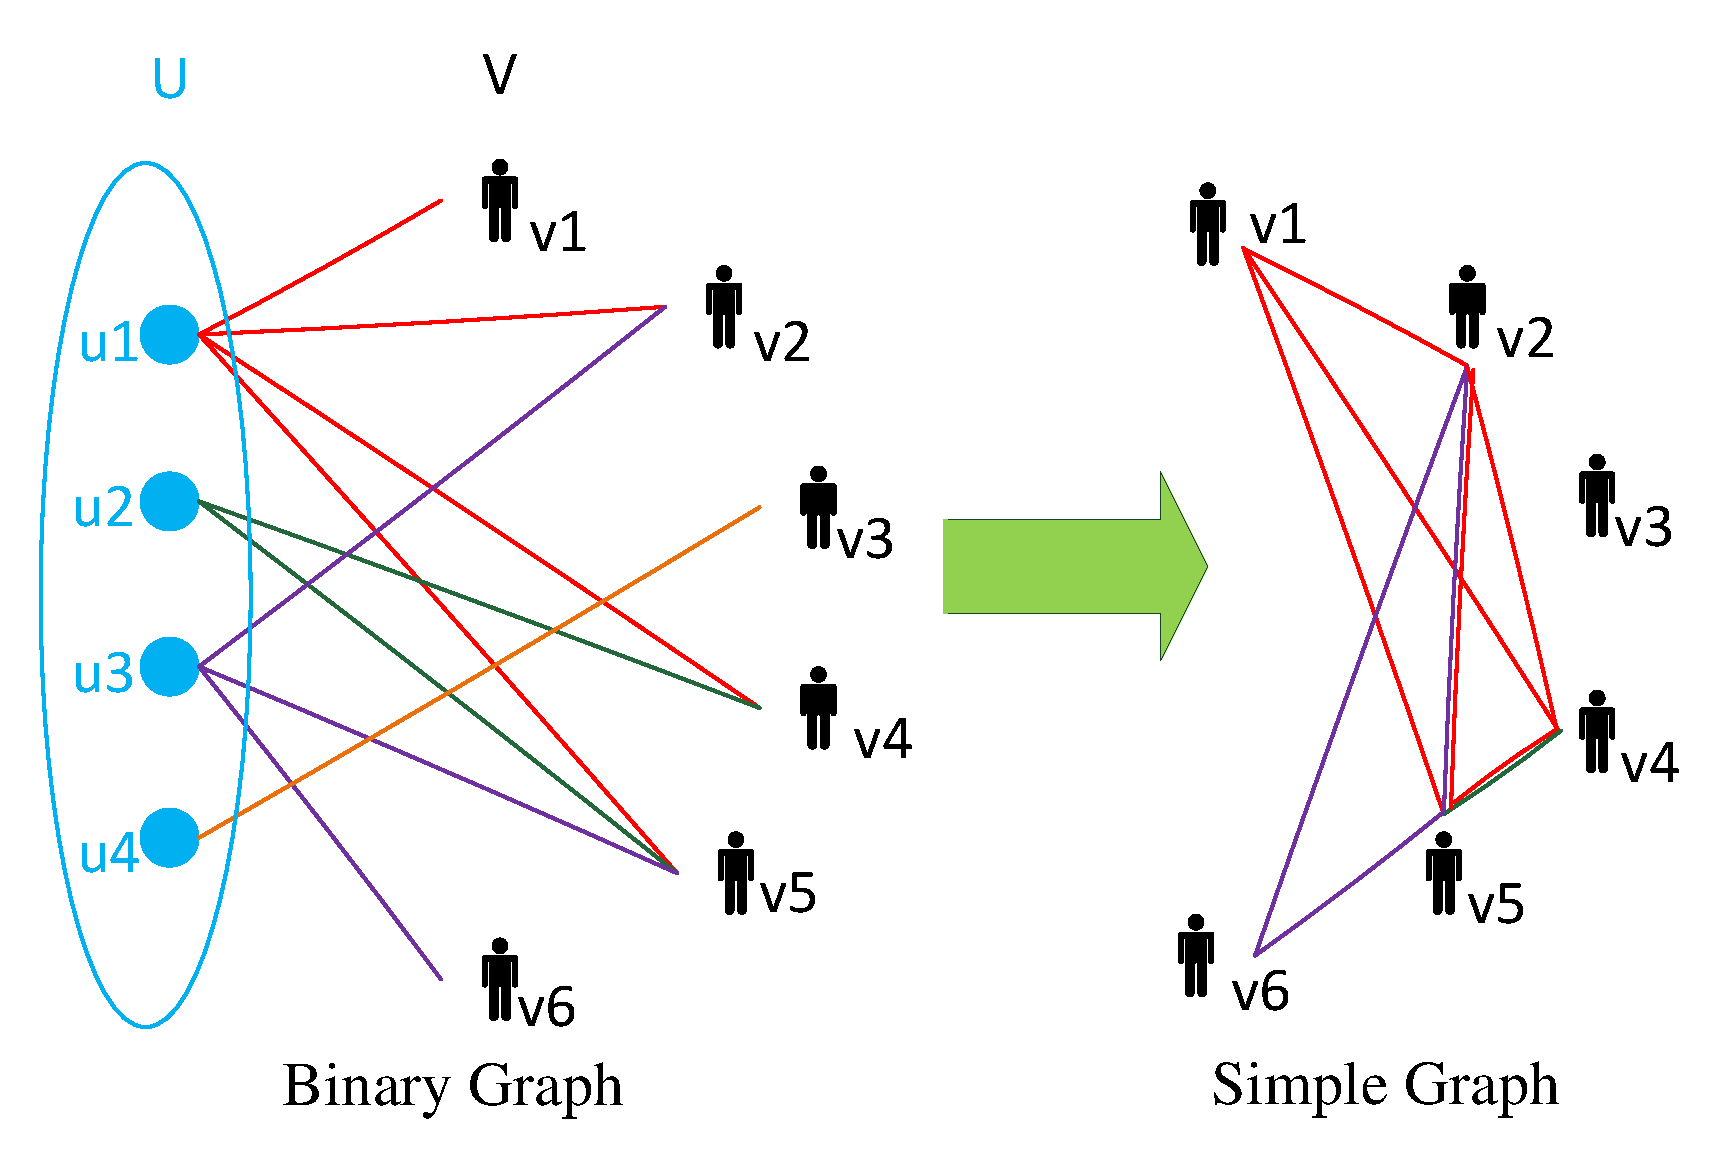
\includegraphics [width=3.5in]{Fig1.pdf}
\caption{Extraction from a Binary Graph to a Simple Graph. $U$ is a list of papers, $V$ is the list of authors. The figure shows three cases: (1) If a scholar has no collaborator, he/she is an isolated node, just like $v_{3}$; (2) If two authors coauthor a paper, there is a link between them, such as $(v_{1}, v_{2})$ and $(v_{6}, v_{5})$. (3) If two scholars coauthored multiple papers, the number of links between them increases, like $(v_{2}, v_{5})$ and $(v_{5}, v_{4})$.}
\end{figure}

In this paper, we propose a novel random walk model named MVCWalker for recommending the most valuable collaborators to scholars, which explores the use of academic factors. This paper substantially extends our previous preliminary work in this line \cite{Jing:ACRec}. MVCWalker is a kind of Random Walk (RW) model in which the rich information of both nodes and links are taken into account when being used for recommendation technology \cite{Backstrom:Supervised}. Random Walk with Restart (RWR) is a classic instance of RW model, which can provide a good relevance score between two nodes in a weighted graph, it has been successfully used in numerous settings, such as personalized PageRank and social recommendation \cite{tong2006fast}. Hence, we take advantage of RW model, by utilizing RWR and optimizing it through guidance for the random walker on the coauthor networks. Additionally, we define link importance based on some academic factors (i.e. the latest collaboration time point, the times of collaboration and the coauthor order). We further explore these three factors to measure co-authors' link importance. This can provide the random walk with more possibility to visit the MVCs on a weighted network and help improve the recommendation quality and accuracy.

In summary, we make the following contributions in this paper:
\begin{itemize}
\item To deal with scientific collaborator recommendation in the context of big scholarly data, we develop a model based on random walk with restart that learns how to bias a random walk on the network so that it can visit the potential collaborators with higher probability than others.
\item In order to improve the recommendation quality and accuracy, we propose and define the link importance of researchers in academic social networks by exploiting three specific factors including coauthor order, the latest collaboration time and collaboration times.
\item We conduct extensive experiments on DBLP data set to evaluate the performance of the proposed method in various scenarios and compare it to RWR and FOF. Promising results are presented and analyzed.
\end{itemize}

The remainder of the paper is structured as follows. Section 2 briefly surveys the related work regarding of social recommender systems, features of coauthor networks, link prediction and RWR. We discuss the details of our proposed model in Section 3, which highlights our problem statement, workflow and computation of link importance. In Section 4 we discuss our experimental settings and analyze the results achieved. Finally, Section 5 concludes the paper.


\section{Related Work}

\subsection{Academic Social Recommender Systems}
Social networks have been studied for decades in an effort to comprehend the relationships between people and detect patterns in such interactions \cite{Barabasi:linked}. Recently much research work has been done on how to utilize social network information to improve recommender systems \cite{Freyne:Social, He:SNRS}. For instance, Ma \textit{et al.} \cite{Ma:Recommender} elaborated on how social networks information can benefit recommender systems and provided a general method for improving recommender systems by incorporating social network information. Perugini \textit{et al.} \cite{Perugini:Recommender} suggested that recommendation has an intrinsic social element and is essentially intended to connect people.

In this paper, we specifically aim to recommend MVCs in academic social networks (based on e.g. big scholarly data), which is different from recommending normal friends or items in academic context. Chin \textit{et al.} \cite{chin2012linking} learned how Offline to Online interactions in a conference can help link people together, improve friend recommendations. Lee \textit{et al.} \cite{lee2011recommending} studied how well content-based, social and hybrid recommendation algorithms predicted coauthor relationship, and the result show that a hybrid algorithm combining expertise and social network information outperformed better. Pavlov and Ichise \cite{pavlov2007finding} proposed a method that extracts structural attributes from graph of past collaborations and uses them to train a set of predictors using supervised learning algorithms, these predictors can then be used to predict future links between existing nodes in the graph. Lopes \textit{et al.} \cite{Lopes:Colleboration} considered researchers' publications area and the vector space model to make collaboration recommendation in academic social networks. A search engine for collaboration discovery named Collabseer was proposed in \cite{Chen:CollabSeer}. In academic social networks, to make MVC recommendations, there are many aspects we should consider, the influential of academic collaboration relationships. In this work, we utilize three specific academic factors into consideration.


\subsection{Coauthor Networks}
Scientific collaboration is a complex social phenomenon in research that has been systematically studied since the 1960s. Furthermore, co-authorship is one of the most tangible and well documented forms of scientific collaboration \cite{glanzel2005analysing}. As a kind of complex social networks, coauthor networks have been studied comprehensively. In these networks two scholars are normally connected if they have coauthored one or more papers together. By mapping the electronic database containing all relevant journals in mathematics and neuro-science for an 8-year period (1991-1998), Barabasi \textit{et al.} \cite{Barabasi:evolution} inferred that the dynamic and the structural mechanisms govern the evolution and topology of coauthor networks. They analyzed the basic network properties of academic social networks in terms of  degree distribution, average separation, clustering coefficient, average degree and so on. Their results indicated that the scientific collaboration network is scale-free, and that the network evolution is governed by preferential attachment, affecting both internal and external links.

Newman \cite{Newman:scientific} studied a variety of statistical properties of scientific collaboration networks, including the number of papers written by authors, numbers of authors per paper, numbers of collaborators that scientists have, existence and size of a giant component of connected scientists, and degree of clustering in the networks. At the same time Newman \cite{Newman:scientific} found out that  a number of differences are apparent among the fields studied. Researchers in different disciplines have different numbers of collaborators on average and the degrees of network clusters are also different.

Coauthor networks can be regarded as rich-information and weighted graphs that can fit many famous models. Liu \textit{et al.} \cite{liu2005co} conducted a coauthor network, for which he defined AuthorRank as an indicator of the impact of an individual author in the network. Their results show clear advantages of PageRank and AuthorRank over degree, closeness and betweenness centrality metrics.
Based on these information of coauthor networks and theoretical support, we propose our model and design our metrics.

\subsection{Link Prediction}
We can formalize academic collaboration recommendation as a link-prediction problem. Many approaches have been proposed for various link predictions \cite{Liu:linkprediction}. For instance, David \textit{et al.} \cite{LN:linkprediction} defined the link-prediction problem as follows: given a social network at time $t$, how to accurately predict the edges that will be added to the network in the future time $t'$. They developed approaches to link prediction based on measures for analyzing the "proximity" of nodes in a network. Their approaches were applied to large social networks and the results suggested that fairly subtle measures for detecting node proximity can outperform direct measures.

Lichtenwalter \textit{et al.} \cite{Lichtenwalter:new} examined important factors for link prediction in networks and provided a general framework for the prediction task. They cast link prediction as a problem in class imbalance. As a result, their  consideration of some important factors leads to a general framework that outperformed unsupervised link prediction methods.

The work more closely related to ours is \cite{Brandao:using}, which emphasizes recommending academic friends and considering the link semantics. The authors proposed two new metrics respectively representing the institutional affiliation and the geographic location of the researchers for recommending new collaborators. Our work differs from \cite{Brandao:using} in that we consider the details of coauthor relationship.

\subsection{Academic Random Walk Model}
Random walk model is often used in daily recommendation scenarios, etc. Mohsen \textit{et al.} \cite{Jamali:trustwalker} proposed a random walk model that combines the trust-based and collaborative filtering approaches for recommendation. They took advantage of random walk to define and measure the confidence of a recommendation. Fouss \textit{et al.} \cite{Fouss:RW} presented a new perspective of characterizing the similarity among elements of a graph. Their method was based on a Markov-chain model involving random walk through the database. In this paper, our work stand on the shoulder of RWR, a famous random walk model, which provides a good way to measure how closely related two nodes are in a graph \cite{Tong:RWR}. It has been successfully used in numerous areas including e.g. collaborative recommendation and link prediction. Konstas \textit{et al.} \cite{konstas2009social} created a collaborative recommendation system that adopts the generic framework of RWR in order to provide with a more natural and efficient way to make recommendation. They conduct some comparative experiments between RWR and CF (collaborative filtering). Their experimental results show that the graph model benefits from the additional information embedded in social knowledge and outperforms the standard CF method. Backstrom \textit{et al.} \cite{Backstrom:Supervised} proposed a supervised random walk based on RWR, to predict and recommend links in social networks.

These studies are quite close to our previous work ACRec \cite{Jing:ACRec}. The main goal of ACRec is to model both the attributes of authors and co-authorship at recommended MVCs so that further recommendation can be generated for researchers. In this paper, we extend ACRec, inject academic factors and build MVCWaler to guide random walk. We conduct much more extensive experiments in this paper than those on ACRec. We examine the influence of two more parameters, iteration times in random walking process and partition of training and testing data sets. We perform further optimizations over the settings of these two parameters. In addition, to further verify the superiority of our method, we compare MVCWalker to both the basic RWR and the popular FOF model in this paper.

\section{Design of MVCWalker}
In this section, we describe the details of MVCWalker. Following problem statement, we give an overview of MVCWalker. Furthermore, we explain how to compute the link importance by considering the academic factors one by one. The symbols used in this paper are listed in Table 1.
\begin{table}
\renewcommand{\arraystretch}{1.2}
\caption{List of Symbols}
\label{tab:1}
\begin{tabular*}{3.5in}{@{\extracolsep{\fill}}r| l}
\hline
Symbol & Definition  \\
\hline
$MR$	           & \multirow{1}{2.8in}{$N\ast1$ ranking score vector}	                             \\
$p_{i}$            & \multirow{1}{2.8in}{Node $p_{i}$} 	                      \\
$L(p_{i})$	           & \multirow{1}{2.8in}{Number of all the neighbors of node $p_{i}$}                           \\
$M(p_{i})$	           & \multirow{1}{2.8in}{Set of nodes incident to node $p_{i}$}             \\
\multirow{2}{*}{$\alpha$}	  & \multirow{2}{2.8in}{Damping coefficient: the probability of a walker walking to the next neighbor}                        \\
~~	   & ~~                       \\
$N$	   & \multirow{1}{2.8in}{Total number of nodes in a graph}    \\
$\mathbf{S}$	   & \multirow{1}{2.8in}{Transfer matrix}   \\
$q$	   & \multirow{1}{2.8in}{$N\ast1$ initial vector of $MR$}	                                     \\
$t$  & \multirow{1}{2.8in}{Iteration times}  \\
$LIM(p_{i}, p_{j})$  & \multirow{1}{2.8in}{Link importance of $p_{i}$ and $p_{j}$}               \\
$DCL(p_{i}, p_{j})$  & \multirow{1}{2.8in}{Distance in coauthor list of $p_{i}$ and $p_{j}$ }	                 \\
\multirow{2}{*}{$k(t)$}	   & \multirow{2}{2.8in}{A monotonically increasing function defined by coauthoring time}                \\
~~	   & ~~                       \\
$P$	   & \multirow{1}{2.8in}{Precision of the recommendation result}                      \\
$R$	   & \multirow{1}{2.8in}{Recall rate of the recommendation result}	                                                 \\
$c$    & \multirow{1}{2.8in}{Coverage rate of the recommendation result}	                                             \\
\hline
\end{tabular*}
\end{table}


\subsection{Problem Statement}

In this paper, our goal is to find and recommend collaborators to researchers. According to Section 2, the aforementioned research efforts exploit collaboration recommendation systems by considering various information in big scholarly data. Some factors will be helpful when making collaboration recommendation based on academic social networks. In addition, the random walk model can be adopted for its remarkable characteristic of integrating the rich information of both nodes and links. In particular, we are targeting the following problems.

\textit{Problem 1}: Academic collaboration recommendation is different from the traditional social recommendation. Scholars need collaborators who have common research interests, valuable and connectable. To recommend MVCs to a scholar, what factors should be considered? How can a recommendation algorithm (or model) be designed to achieve this goal?

\textit{Problem 2}: As mentioned in Section 1, social interactions and its relational aspects can help recommend collaborators. Various academic social network features could be considered. However, what relations are featured in academic social networks? What features are available?

%\Statement bbbbbb
\subsection{Overview of MVCWalker}
The MVCWalker collaborator recommendation model is inspired by the truth that scholars usually desire to co-operate with people who have high academic value. Such people normally have fruitful high-quality papers, which can generally be used to represent their academic achievements. Besides, as the RWR model has been proved to be competent for calculating the similarity of nodes in network, we use it as a basic model for the coauthor social network. Furthermore, we introduce edge attributes information into the network structure to bias the random walk such that it will more easily traverse to the positive nodes.

In MVCWalker recommendation, finding one's MVCs depends on the importance of other nodes to the target node. According to the importance, each recommended node has a rank score, which is determined by two factors, the number of nodes connected to this node and the importance of these nodes. It can be described as:
\begin{equation}
MR(p_{i})=\frac{1-\alpha}{N}+\alpha \sum_{p_{j}\in M(p_{i})}\frac{MR(p_{j})}{L(p_{j})}
\end{equation}
where $MR$ represents the rank score vector, and $MR(p_{i})$ is the rank score of node $p$, which is the quantized importance of node $p_{i}$ to the target node. $M(p_{i})$ is the set of nodes incident to node $p_{i}$, with $L(p_{j})$ being the number of all the neighbors of node $p_{j}$. $\alpha$ denotes the probability that the walker will continue to walk to the next neighbor. Above all, in MVCWalker model, the walker has the probability to randomly skip to any other nodes. Equation (1) represents only the step to get the rank score of a node. With respect to each node in the whole graph, the personalized random walk process is defined by (2), which is an iterative process.

\begin{equation}
MR^{(t+1)}=\alpha \mathbf{S}MR^{(t)}+(1-\alpha)q
\end{equation}
where $\mathbf{S}$ is the transfer matrix, representing the probability for each node to skip to other nodes. $MR^{(t)}$ represents the rank score vector at step t, and $q$ is the row vector, and its form is $(0, \ldots, 1, \ldots, 0)$. In fact, at the beginning, $MR^{(0)}=q$, and the rank score of target node is 1, while others' are 0.

Consider a single random walker that starts from node $p_{i}$. The walker iteratively transmits to its neighborhood with the probability $\alpha S_{i,j}$, which is proportional to their link importance. At each step, it has the probability of $(1-\alpha)q_{i}$ to return to node $p_{i}$.

The relevance score defined by MVCWalker has many good properties: as compared with those common neighbor models, it can capture the global structure of a graph; while compared with those traditional short distance models, it can capture the multi-facet relationship between two nodes \cite{Tong:center}.

Basic random walk models usually assume that the weights of edges are the same \cite{tong2006fast}, and define the cells of matrix $\mathbf{S}$ as $S_{i,j}=\frac{1}{L(p_{j})}$. In contrast, here we define matrix $\mathbf{S}$ by link importance based on academic factors. We will introduce the link importance in Section 3.3.

The detailed process of MVCWalker is described below and the corresponding pseudocode is shown in Algorithm 1. The structure of MVCWalker is illustrated in Fig. 2.
\begin{figure}
\centering
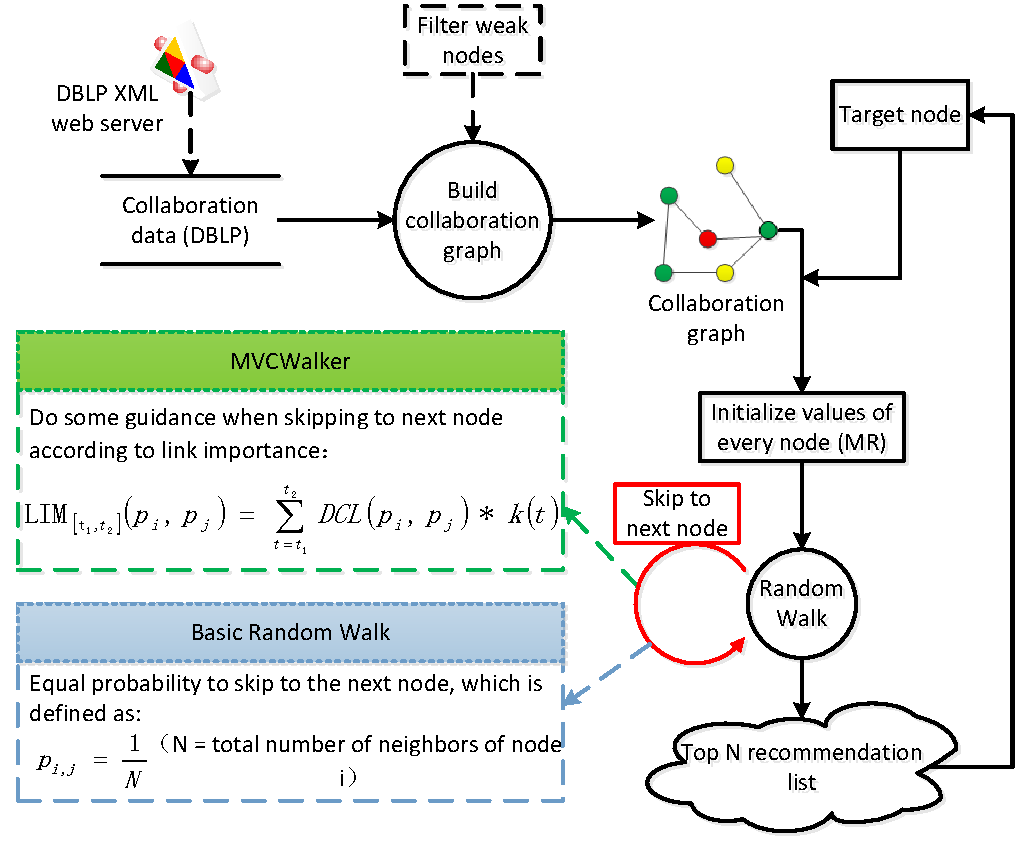
\includegraphics [width=3.5in]{Fig2.pdf}
\caption{Structure of MVCWalker.}
\end{figure}
\begin{itemize}
\item The initial input data of MVCWalker is a set of several years' papers published by many scholars. To extract the coauthor network, we regard authors as nodes in the network. Before that, it is necessary to filter out the isolated nodes and weak nodes (with small degree). We define the graph $G$ as the coauthor network, and $P$ as the set of the nodes.
\item If some authors have worked for one publication together, add edges among all those authors, which are defined as set $E$. In this step, we calculate the weight of each edge which is called the link importance in MVCWalker. Some attributes of collaboration should be taken into account (e.g. coauthor order, latest collaboration time point, and collaboration times), which will be described in the next section. We define the link importance between the nodes $P_{i}$ and $P_{j}$ as $LIM(P_{i},p_{j})$.
\item Before starting the random walk, we need to acquire the transfer matrix $S$ as described in Algorithm 1. To be specific, we denote $P_{i}$ as the current node while $P_{j}$ as the next node. $\mathbf{S}$ is the set of probabilities for each $P_{i}$ in $G$ skipping to next node $P_{j}$. This can be described as $S_{i,j}=\frac{LIM(P_{i},p_{j})}{\sum_{P_{k}\in M(P_{i})} LIM(P_{i},p_{k})}$, while $M(P_{i})$ is the set of neighbors of $P_{i}$.
\item MVCWalker starts with initializing the rank score vector $MR^{(0)}$ and the restart probability vector $q$ as (0,\ldots,1,\ldots,0). The target node $P_{i}$ is set to 1 while others are set to 0. MVCWalker iterates the traversal starting with node $P_{i}$ until random walk stops walking and assigns each candidate node $P_{k}$ a stable probability $MR(p_{k})$. Thus we get the rank score vector $MR$. Then sort the nodes in accordance to their corresponding rank scores.
\item Finally, the Top N nodes in the $MR$ list are recommended to the target nodes. Of course, we can take out the nodes which have been in its coauthor list before recommending. That is the new co-authors recommendation.
\end{itemize}

\begin{algorithm}
  \caption{MVCWalker(R, a, MaxIteration, MinDelta)}
  \begin{algorithmic}[1]
    \State $\mathbf{S}\leftarrow$ ComputeTransferMatrix()
    \State $MR_{0} \leftarrow R$
    \State $Q \leftarrow R$
    \For {$k \leftarrow 0$~to~$MaxIteration-1$}
        \State $diff \leftarrow 0$
        \For {$i \leftarrow 0$~ to~$len(Q)-1$}
            \State $MR_{k_{i}} = \alpha\sum_{j=0}^{len(Q)} S_{i,j}MR_{j}+(1-\alpha) Q_{i}$
            \State $diff \leftarrow diff +(MR_{k}-MR_{k-1})$
        \EndFor
        \If {$diff<MinDelta$}
            \BREAK
        \EndIf
    \EndFor
    \State $Predictions \leftarrow predictions(MR)$\\
    \Return $Predictions$
  \end{algorithmic}
\end{algorithm}

We present below the details of how the link importance is computed by taking into account the three academic factors.

\subsection{Link Importance}
As mentioned in Fig. 1, when extracting a simple graph from a binary graph, considering the information about link features will be better, which indicate the importance of cooperation relationship between nodes. In reality, people might be more willing to choose certain nodes with high feature value for them. Therefore, a critical requirement of the MVC recommendation algorithm is to assign cooperation graph edge with related weight, to measure the cooperation relationship strengths between one user and his/her (potential) collaborators. We define the edge weight as \emph{LIM} (Link Importance of MVCWalker).

Common sense depicts that, when choosing a collaborator, a scholar might prefer a researcher with whom he/she coauthored papers within the past year, rather than ten years ago. Consequently it seems that, closer relationships between authors are established through frequent collaboration, because coauthored papers can reflect the interest similarity of the authors. Even the coauthor order can reflect the similarity of the authors to some extent. This is why we choose these three factors, coauthor order, latest collaboration time point, and times of collaboration, to calculate LIM.

\subsubsection{Coauthor Order}
There is always a list of (co)authors for one paper. Normally, their contributions to the paper differ from each other, which we can measure generally by the author order. For example, the first two authors usually make more contributions than the rest authors. In such cases, the cooperation relationship between the first two authors is competently strong. That is, the coauthor order can reflect cooperation relationship strength. As a general rule, the contribution value is inversely proportional to the coauthor order, and the weight of relationship is contributed by the relevant two nodes. Therefore, we propose a measure of the link importance based on the coauthor order: \emph{DCL} (distance in coauthor list).

Consider two nodes $p_{i}$, $p_{j}$ in a coauthor list. Assume that $j > i$, and there are more than one author of a paper. For the sake of simplicity, we calculate $DCL(p_{i}, p_{j})$ as follows.

\begin{equation}
DCL(p_{i}, p_{j})=\left\{\begin{array}{ll}
\frac{1}{i}+\frac{1}{j} & j\leq 3\\
\frac{1}{i}+\frac{2}{j} & j>3, i\leq 3\\
\frac{2}{i}+\frac{2}{j} & i>3
\end{array}\right.
\end{equation}
According to this definition, it is clear that the $DCL$ value between the first and the second authors is 1.5, which is the maximum. The relationship between first two authors is the closest, while the relationship between the first author and the rest authors is relatively weak.

\subsubsection{Latest Collaboration Time Point}
In recent years, more and more social recommendation systems introduced time dependence models (e.g. \cite{toscher2009bigchaos}). Especially, academic social networks are obvious time-varying, where the links among scholars change over time. For instance, scholars might be more willing to collaborate with whom coauthored a paper last year, as compared to the co-authors of ten years ago. Hence, we measure the link dynamics using $LIM_{t}(p_{i}, p_{j})$ (i.e. Link Importance):

\begin{equation}
LIM_{t}(p_{i}, p_{j})=DCL(p_{i}, p_{j})\ast k(t)
\end{equation}
To reflect the dynamic feature of coauthor-ship, we introduce the equation $k(t)$, a monotonically increasing function over time. We can measure the impact of different coauthoring time points by adjusting the parameter $k(t)$. Here, we define $k(t)$ as:
\begin{equation}
k(t)=\frac{t_{i}-t_{0}}{t_{c}-t_{0}}
\end{equation}
where $t_{i}$ is the published time of the paper $i$ two researchers coauthored (in year here), $t_{c}$ is the current time (i.e. 2014 in this paper) and $t_{0}=Published\ year\ of\ the\ first\ coauthored\ paper-1$. In fact, this is a process of normalization. The experimental results in section 4 demonstrated its effectiveness.

\subsubsection{Times of Collaboration}
In academic social networks, if two authors coauthor a paper, there will be a link between them. Furthermore, these two authors may collaborate many times. It is necessary to take the times of collaboration into account when measuring the link importance between two authors. Here we measure the impact of different times of coauthoring as follows:
\begin{eqnarray}
LIM_{[t_{1}, t_{2}]}(p_{i}, p_{j})&=&\sum_{t=t_{1}}^{t_{2}}LIM_{t}(p_{i}, p_{j}) \nonumber\\
                       &=&\sum_{t=t_{1}}^{t_{2}}DCL(p_{i}, p_{j})\ast k(t)
\end{eqnarray}

According to above equation, we will calculate the sum of each link importance if there are $n$ links between $p_{i}$ and $p_{j}$ during time period $t_{1}\sim t_{2}\ (t_{0} < t_{1}\leq t_{2} < t_{c})$.

\subsection{An Example}

\begin{table}
\renewcommand{\arraystretch}{1.2}
\centering
\caption{Seven papers by five researchers}
\begin{tabular}{|c|c|c|c|} \hline
Paper ID&Authors&Published year\\ \hline
1 & Alice, Bob, Charlie, David &2009 \\ \hline
2 & Bob, Eden &2010 \\ \hline
3 & Alice, Charlie, David &2013 \\ \hline
4 & Eden, David, Bob &2012 \\ \hline
5 & Bob, David, Alice, Charlie &2013 \\ \hline
6 & Charlie, Bob, Alice &2014 \\ \hline
7 & Bob, Eden, David &2011 \\ \hline

\hline\end{tabular}
\end{table}
As shown in Table 2, there are seven papers created by five researchers including paper id, orderly authors and published year. We can get the coauthor network (Fig. 3.) according to the coauthor activities, and then, calculate the LIM by making full use of these information. e.g. David and Eden have coauthored two papers (4 and 7) in 2011, 2012. The authors order are respectively (2, 1) and (3, 2). According to equation (6) and these data from their first cooperation time to now, We can compute that the LIM of David and Eden is $\frac{17}{12}$. Similar to the other authors, we can get the LIM values of all coauthor relationships, which have been displayed in Fig. 3.

Assume that we make some academic cooperation recommendations for Eden. We know that she has two co-authors now, Bob and David. Regarding Eden as a random walker with initial $MR$ value 1 (others 0), when deciding next jump, she has two equiprobable choices in basic RWR model, i.e. 0.5 probability to Bob and 0.5 probability to David. In MVCWalker model, we utilize a guidance procedure for this decision making process. She has probability of $0.602$ (i.e. $\frac{77/36}{17/12+77/36}$) jumping to the node Bob, and $0.398$ (i.e. $\frac{17/12}{17/12+77/36}$) to node David. The result of our experiment has proved the effectiveness of the guidance work. After limited times of iteration (19 times in this case), each of the nodes have have their own $MR$ values which represent the importance to Eden. In this case, The $MR$ values of Bob, Charlie, David, and Alice are $0.500$, $0.391$, $0.384$, $0.376$ respectively. Hence we know that Bob is the most suitable partners in this circle, and Charlie can be recommended to Eden as a new cooperator (even though Eden has never worked with Charlie).

\begin{figure}
\centering
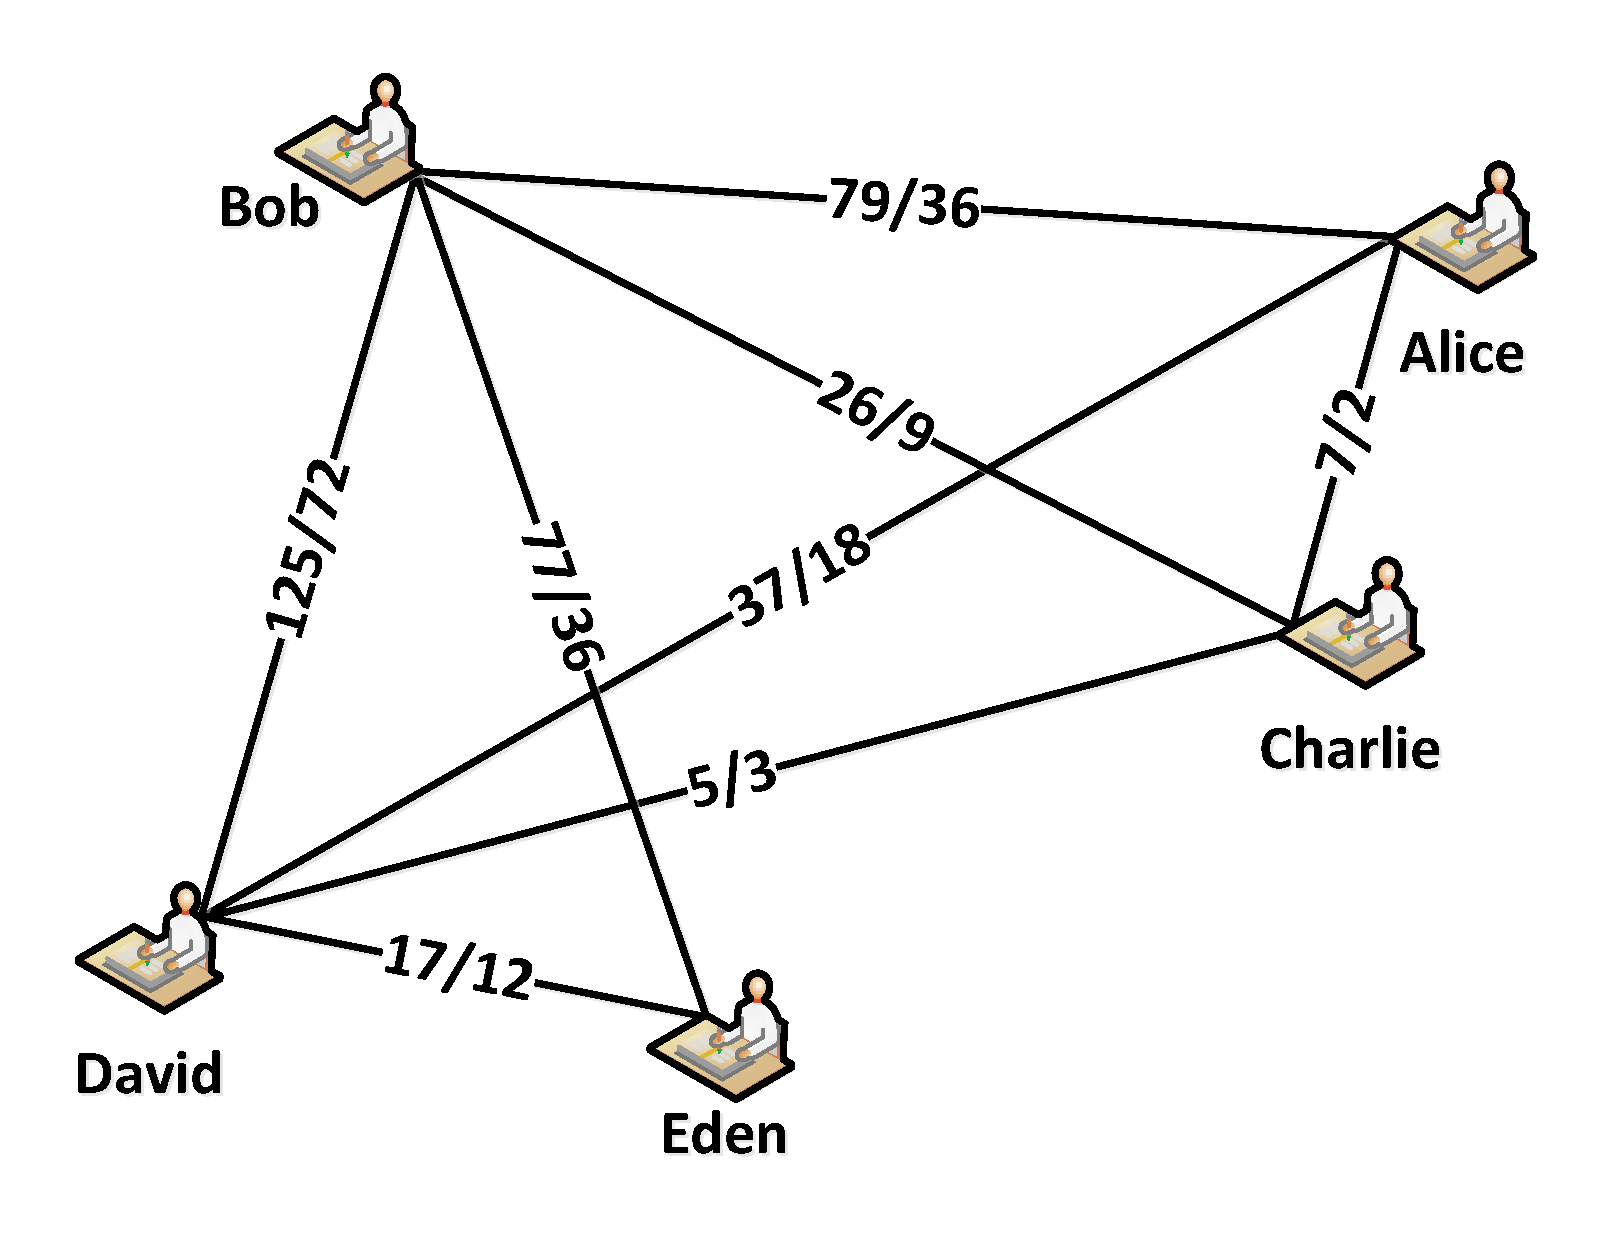
\includegraphics [width=3in]{Fig-example.pdf}
\caption{Coauthor network with link importance over these five researchers}
\end{figure}

\section{Evaluation and Analysis}
We conducted extensive experiments using data from DBLP \cite{Ley:DBLP}. In this section, we describe the processing of DBLP data set, the evaluation metrics we employed and our experimental procedure for evaluating the performance of MVCWalker, as well as detailed analysis of the results.

To improve the effectiveness and efficiency of our MVCWalker model, we examined the influence of different parameters by conducting a series of experiments and optimization of some parameters. Within the same period, we embarked on different experiments to compare MVCWalker to the RWR and FOF models in terms of multiple metrics (i.e. precision, recall rate and coverage rate).

Similar to popular random walk models, the details and verification method of RWR is just like MVCWalker, except for the definition of link importance. FOF is a common neighbor-based model. Its basis of recommending collaborators is the number of common neighbors. For two researchers, the more common neighbors they have, the more suitable to recommend each other.

All experiments were performed on a 64-bit Linux-based operation system, Ubuntu 12.04 with a 4-duo and 3.2-GHz Intel CPU, 4-G Bytes memory. All the programs are implemented with Python.

\subsection{Data Set}

DBLP indexes more than 2.3 million articles on computer science and contains many links to home pages of computer scientists. Generally, each DBLP record contains these attributes, authors, title, pages, years, crossref, (in)proceedings or journals, etc. According to the methods provided by \cite{Ley:DBLP}, we can extract a subset of the entire data set using the required information. The reasons why we use a subset of the data set are as follows.

\begin{itemize}
\item It is possible that the subset of the researchers' publications be represented by a social network \cite{Brandao:using} and the analysis of published papers are of great significance to recommend most valuable collaborators.
\item In a coauthor graph, there are some isolated authors who write publications without any cooperation. Thus, they nearly have no relationship with other scholars. Furthermore, we define these isolated authors as the weak nodes, since their degree values are 0. It is clear that the weak nodes have little impact on the random walk. Therefore, to measure the performance of MVCWalker better, we ignore the weak nodes whose degrees are less than 1.
\end{itemize}

The data sets we extracted are all in the field of data mining involving 34 journals and 49 conferences altogether. The statistics about the data sets are shown in Table 3. The data sets contain 59659 nodes (authors) and 90282 edges (coauthor relations). In additionally, the average degree is 1.513, which indicate that these data sets are very sparse.
\begin{table}
\renewcommand{\arraystretch}{1.2}
\centering
\caption{Statistics of Data Set from DBLP}
\begin{tabular}{|c|c|c|c|} \hline
Statistics &Nodes&Edges&Average Degree\\ \hline
Number & 59659 &90282 &1.513 \\
\hline\end{tabular}
\end{table}

\subsection{Metrics}

We chose three popular metrics, precision, recall rate and coverage rate, to evaluate the performance of MVCWalker \cite{Fouss:web, Shani:recommender}. Usually, the output of a recommendation system including MVCWalker model is a recommendation list. After some time, there will be a new list of co-authors for the target node. We can divide all nodes into four groups according to the following four cases (as shown in Table 4):
\begin{itemize}
\item A: collaborating with target nodes and recommended;
\item B: collaborating with target nodes but not recommended;
\item C: not collaborating with target nodes but recommended;
\item D: not collaborating with target nodes and not recommended.
\end{itemize}
\begin{table}
\renewcommand{\arraystretch}{1.2}
\centering
\caption{Possible Results of Recommendation}
\begin{tabular}{ |c|c|c|} \hline
                 &Recommended &Unrecommended\\ \hline
Collaborated    & A          & B\\ \hline
No collaborated & C          & D\\
\hline\end{tabular}
\end{table}

The metric precision is defined as:
\begin{equation}
P=\frac {A}{\langle A+C \rangle}
\end{equation}

The metric recall rate is defined as:
\begin{equation}
R=\frac {A}{\langle A+B \rangle}
\end{equation}

From the definitions, we can see that the higher precision and recall rate, the better performance.

In this work, we modified the general definition of the metric coverage rate, the average of shortest path from recommended nodes to the target node. We believe that, it will be a pleasantly surprised and interesting recommendation if we get the high "coverage rate", which means we recommend more "file-new" and "wide-selected" possible cooperators to the target researcher.
\begin{equation}
c=\frac {\sum d}{n}
\end{equation}
where $d$ denotes the shortest path from recommended node to target node, and $n$ is the total number of recommended nodes. With this definition, a higher $c$ means a better coverage.

\subsection{Impact of Various Parameters}
In this section, we examine the impact of different experimental parameter settings, including range of target nodes' degree, time point of data set partition, iteration times, damping coefficient and the number of recommended nodes. The ranges and default values of the parameters are summarized in Table 5. When the effect of a parameter is under examination, the other parameters are set to the default values. For each experiments, we randomly chose 100 constant nodes as recommended targets, and compute the average of precision, recall rate and coverage rate. Through the experiments, we can attain the best values of them for later tests.
\begin{table}
\renewcommand{\arraystretch}{1.2}
\centering
\caption{Simulation Parameters}
\begin{tabular}{|c|c|c|}                                                       \hline
Parameter                    & Range                           & Default    \\ \hline
Target nodes' degree         & $\geq 0$           & $\geq 30$          \\ \hline
Partitioning Time Point      & 2008$\scriptsize{\sim}$2012     & 2011       \\ \hline
Iteration times              & 10$\scriptsize{\sim}$100        & 25         \\ \hline
Damping Coefficient          & 0.1$\scriptsize{\sim}$0.95      & 0.8       \\ \hline
Number of recommended nodes  & 5$\scriptsize{\sim}$100         & 10        \\ \hline
\end{tabular}
\end{table}

\subsubsection{Target Nodes' Degree}

\begin{figure*}
\centering
\subfigure[Precision]{
\label{fig:4-a}
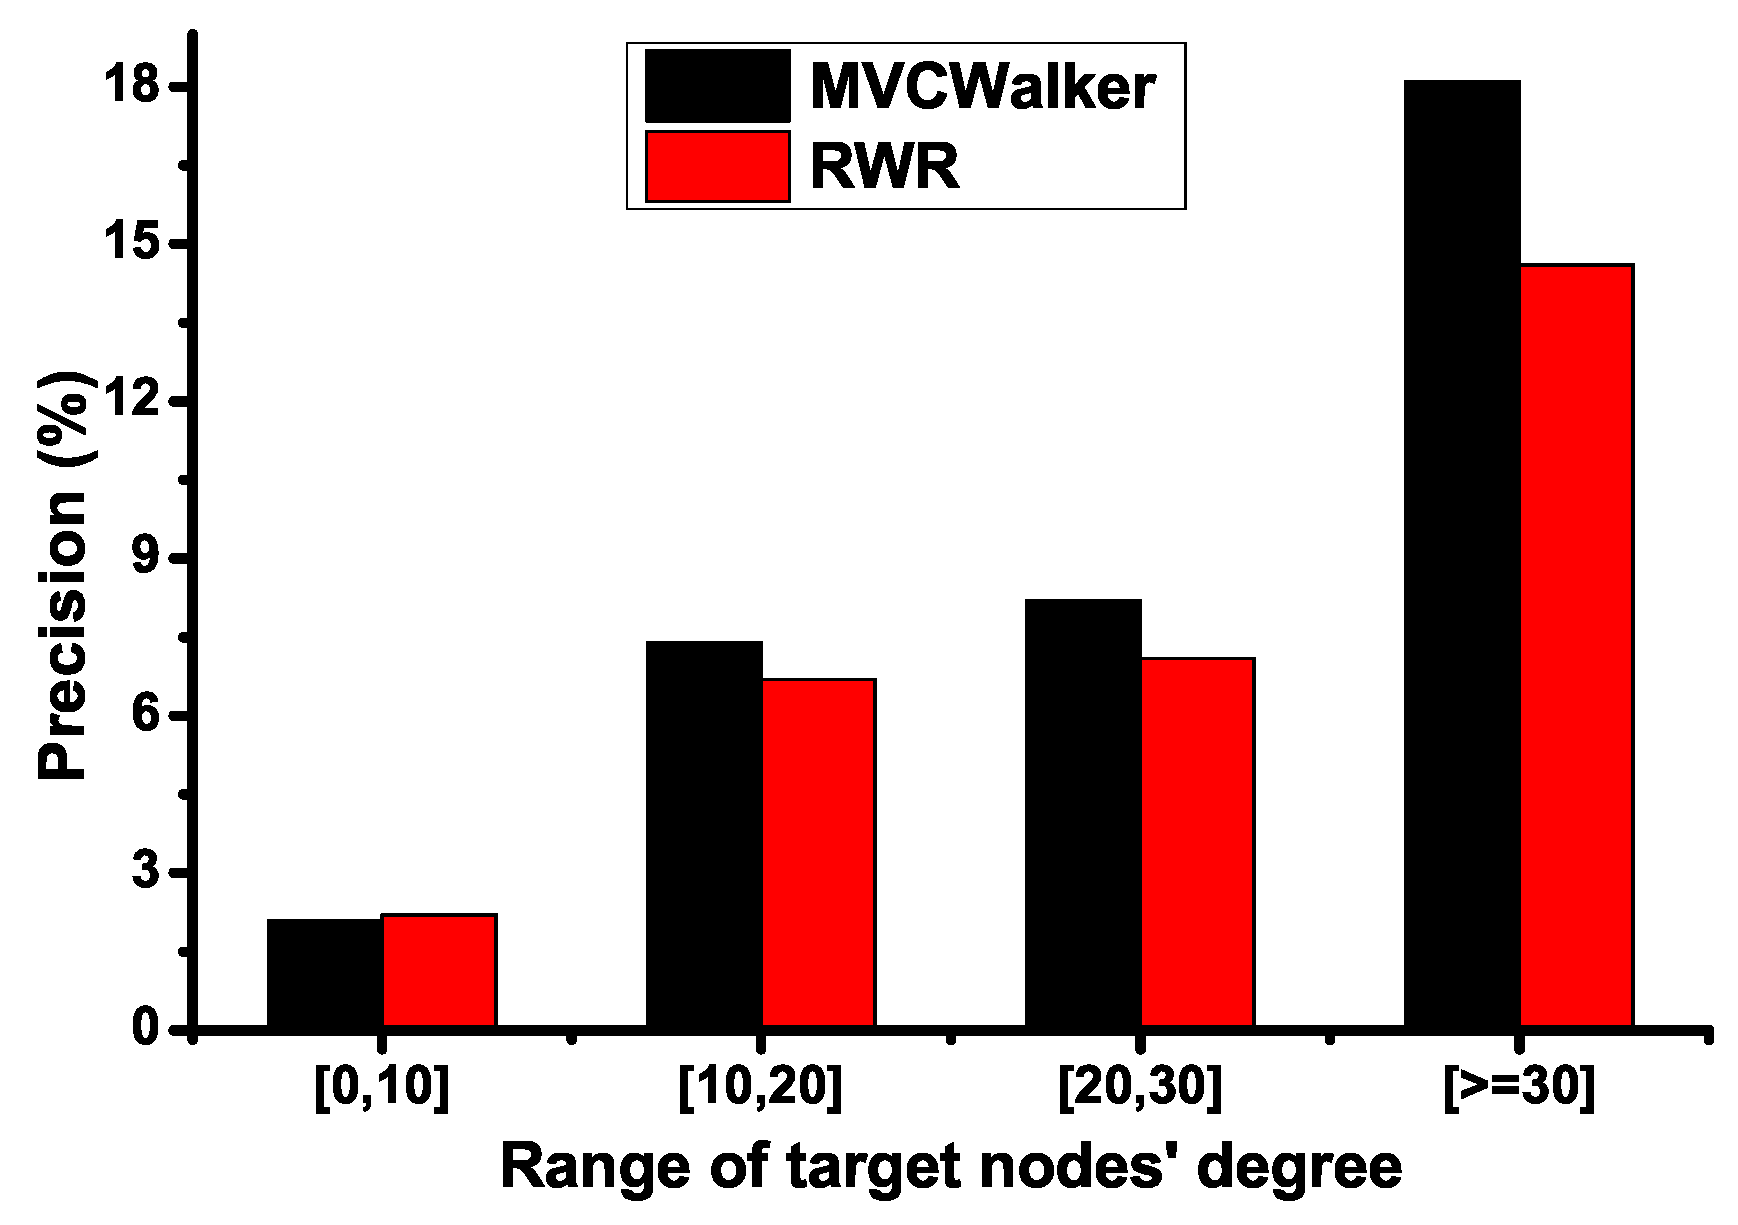
\includegraphics[width=0.31\textwidth]{Fig4-a.eps}}
\subfigure[Recall Rate]{
\label{fig:4-b}
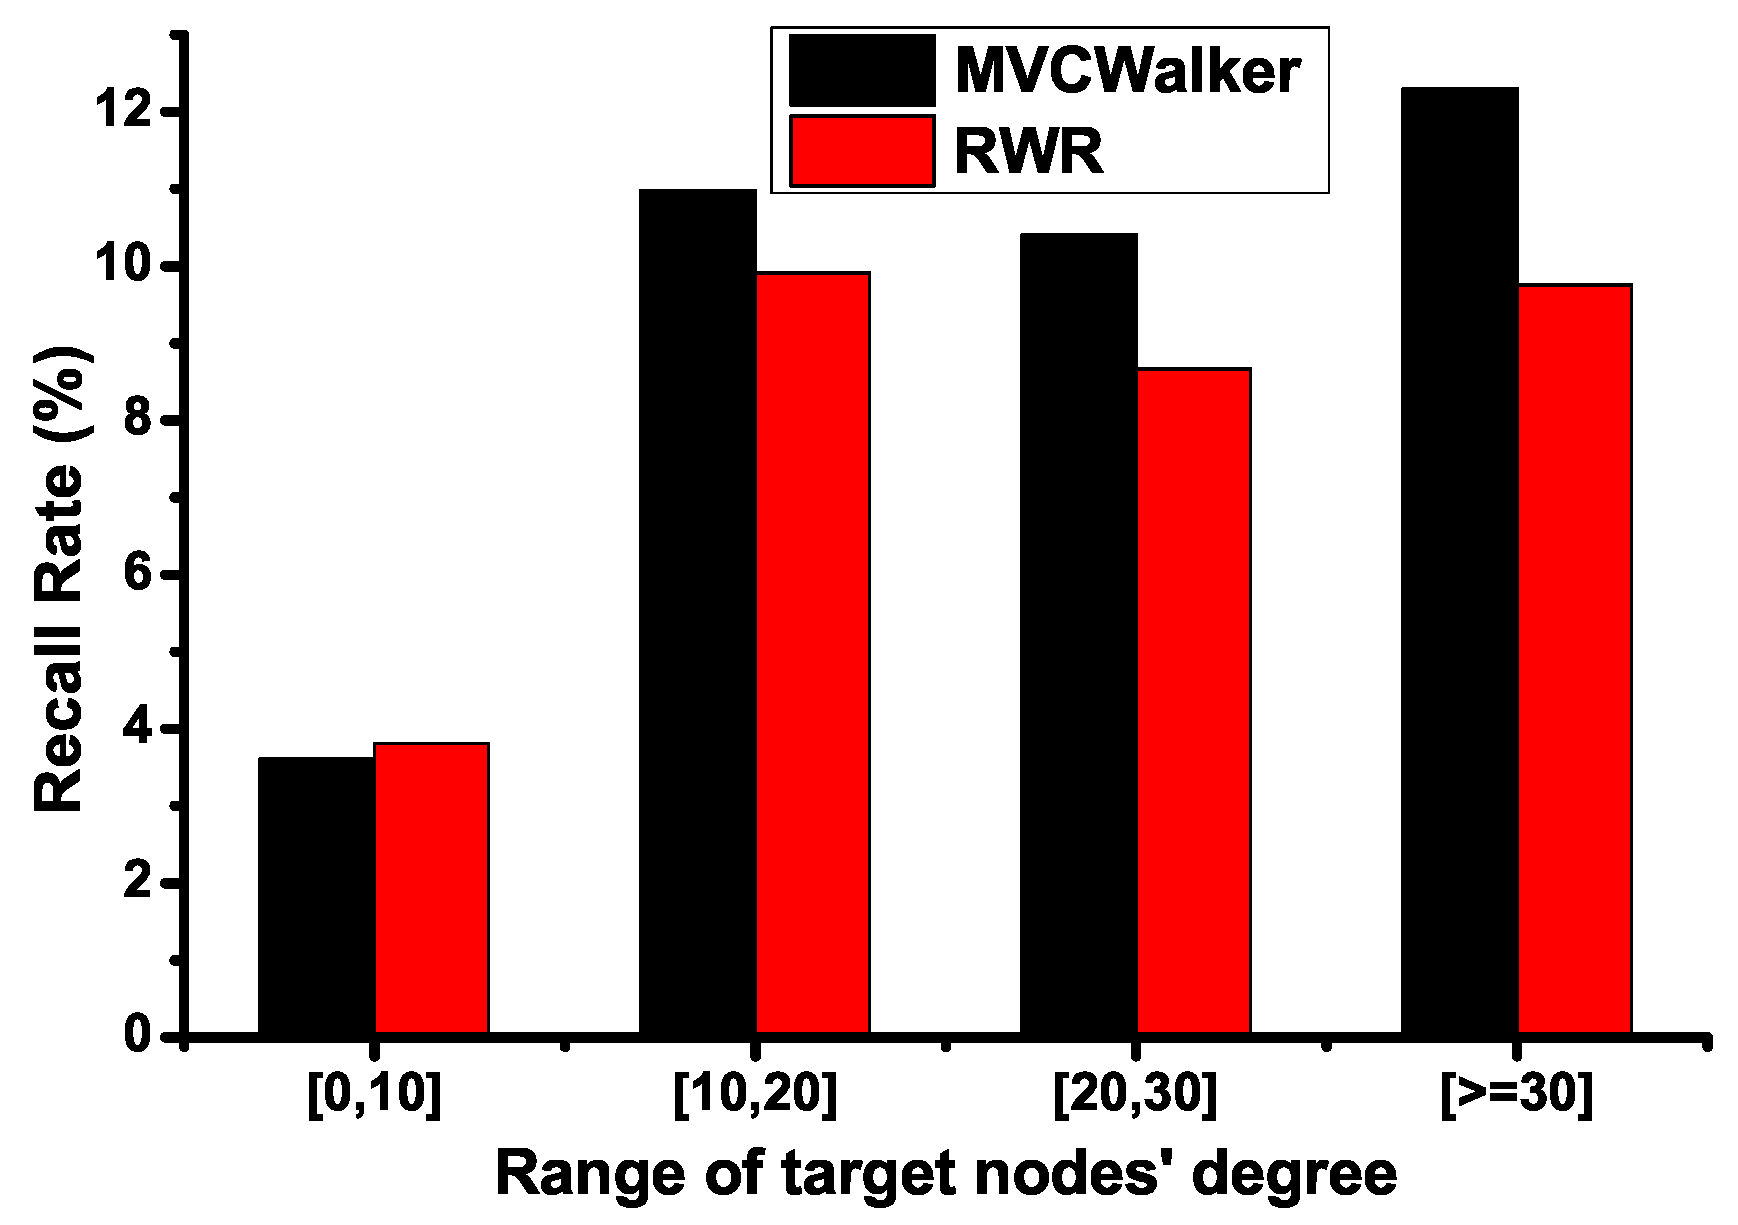
\includegraphics[width=0.31\textwidth]{Fig4-b.eps}}
\subfigure[Coverage Rate]{
\label{fig:4-c}
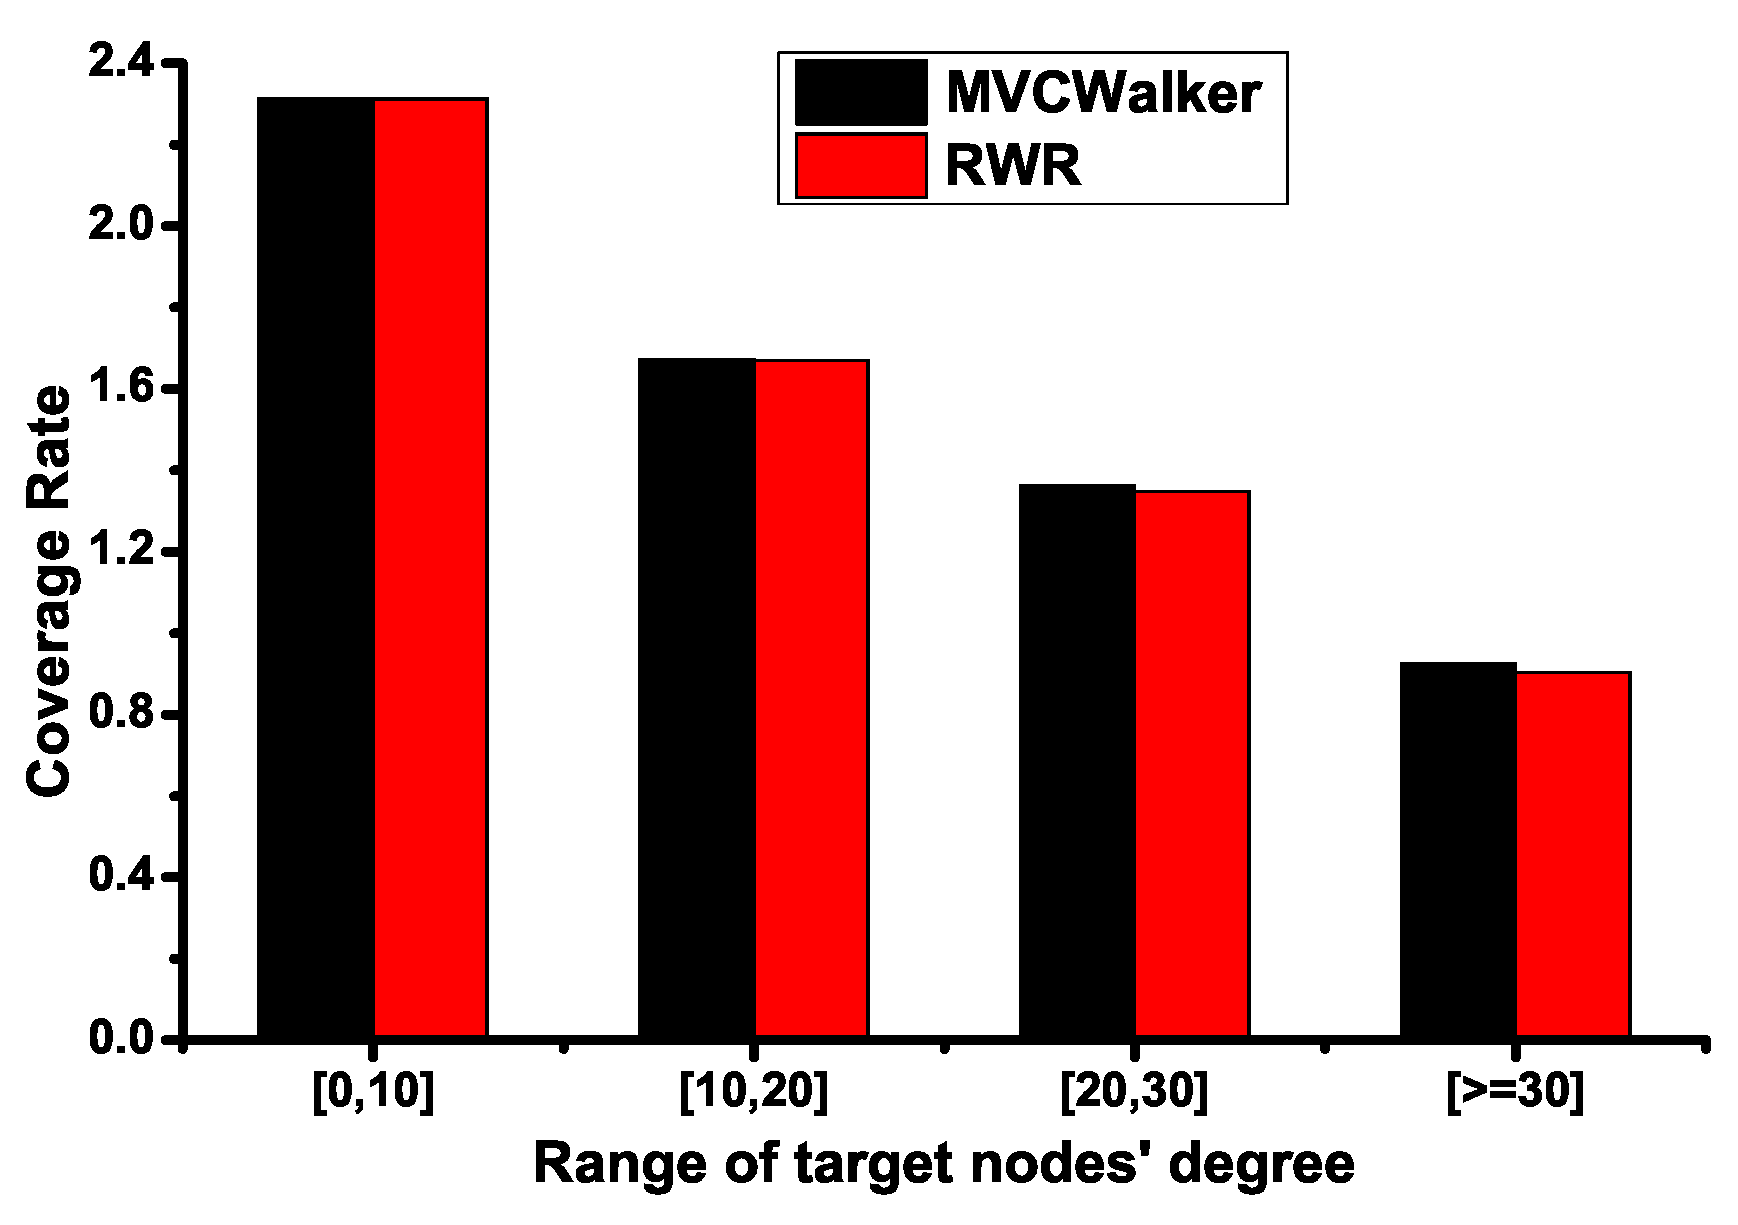
\includegraphics[width=0.31\textwidth]{Fig4-c.eps}}
\caption{Performance of MVCWalker and Basic RWR over Target Nodes' Degree}
\label{fig:4}       % Give a unique label
\end{figure*}
In an academic social network, there are some "strong nodes" and "weak nodes", which are defined by the number of collaborators in our model. Strong nodes have many more collaborators than weak nodes. In other words, the degree of a strong node is larger than that of a weak node. To examine the influence of the target nodes' degree in the experiments, we conduct four experiments in this part. When choosing the 100 target nodes each time, we controlled the degree respectively in range of $0\sim10$, $10\sim20$, $20\sim30$, $>30$. Other parameters are set to the default values as Table 5. The results of the four experiments are displayed in Fig. 4.

As shown in Fig. 4, the target node's degree has an influence on the metrics with a clear trend. From a practical perspective, it is different to recommend co-authors to those who have different number of collaborators. In terms of precision in Fig. 4(a), the larger the target node's degree, the better the model's performance. Besides, we can see that MVCWalker has relatively higher precision than RWR. At the range from 0 to 10, MVCWalker performs similarly to RWR. But when the target node's degree gets larger than 30, the precision can be as high as 18.1\%, much more than RWR. Thus we can conclude that, as compared against RWR, MVCwalker has higher precision for strong nodes, but performs almost the same for weak nodes.

Fig. 4(b) shows the comparison of recall rate with the changing degree. The first two columns are almost the same for recall rate, while the gaps between the two models get larger for other columns. Similar to the results on precision, when the degree becomes larger than 30, the corresponding recall rate of MVCWalker is 12.3\%, much higher than that of RWR (10.4\%). Hence it can be realized that MVCWalker performs better than RWR on recall rate with varying target node's degree.

We can see the effect of target nodes' degree on the coverage rate from Fig. 4(c). The overall trend of coverage is distinct from the former metrics. The values of both models decrease respectively from 2.3 to 0.95 and 2.3 to 0.9. The results indicate that, for weak nodes, the neighbouring network becomes sparser with less valuable information, leading to the random walk going further; while for strong nodes, there are enough valuable nodes to be recommended in the neighbouring network.

This phenomenon is also due to that weak nodes are not so active as strong nodes, and there is not enough valuable information for analysis and making recommendation. The analysis above leads us to the conclusions that MVCWalker outperforms RWR and it can make a better recommendation especially for strong nodes.

\subsubsection{Partition of Training and Testing Data Sets}

\begin{figure*}
\centering
\subfigure[Precision]{
\label{fig:5-a}
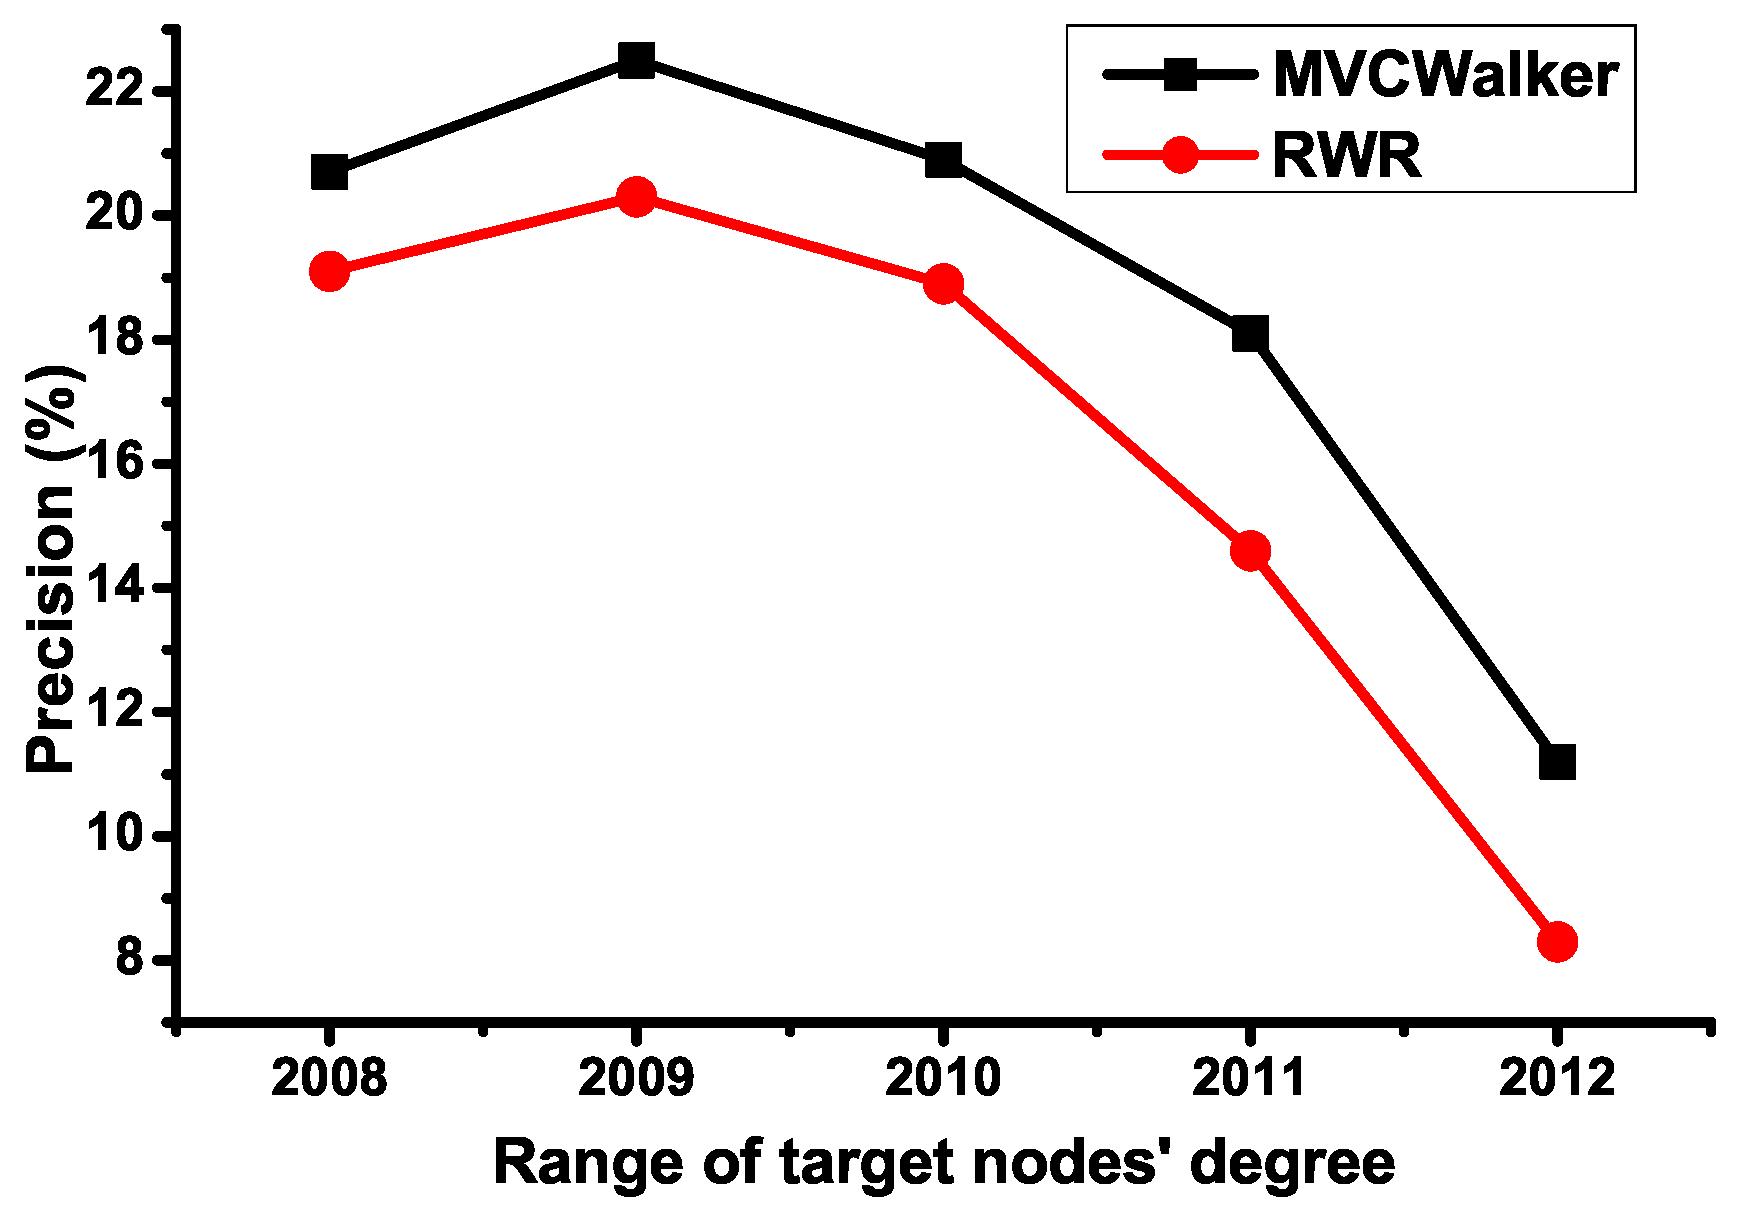
\includegraphics[width=0.31\textwidth]{Fig5-a.eps}}
\subfigure[Recall Rate]{
\label{fig:5-b}
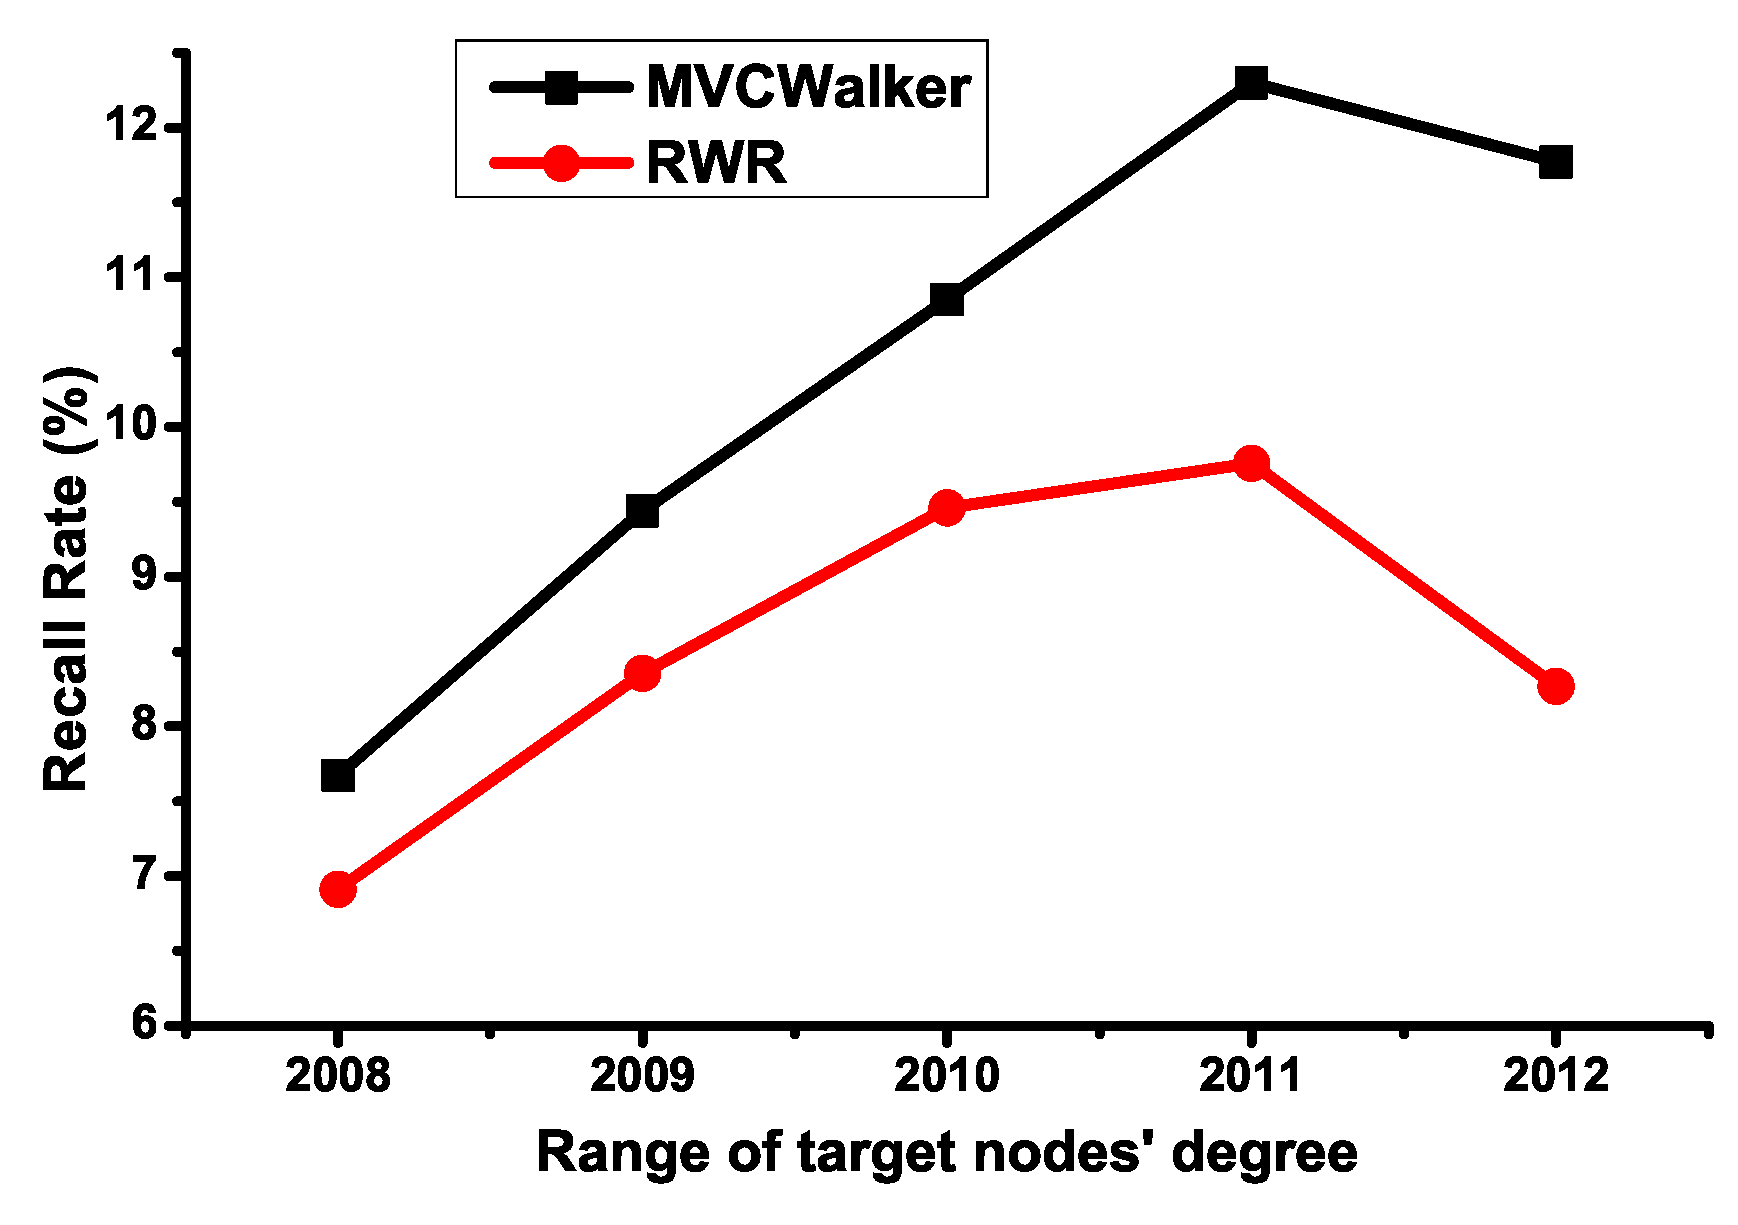
\includegraphics[width=0.31\textwidth]{Fig5-b.eps}}
\subfigure[Coverage Rate]{
\label{fig:5-c}
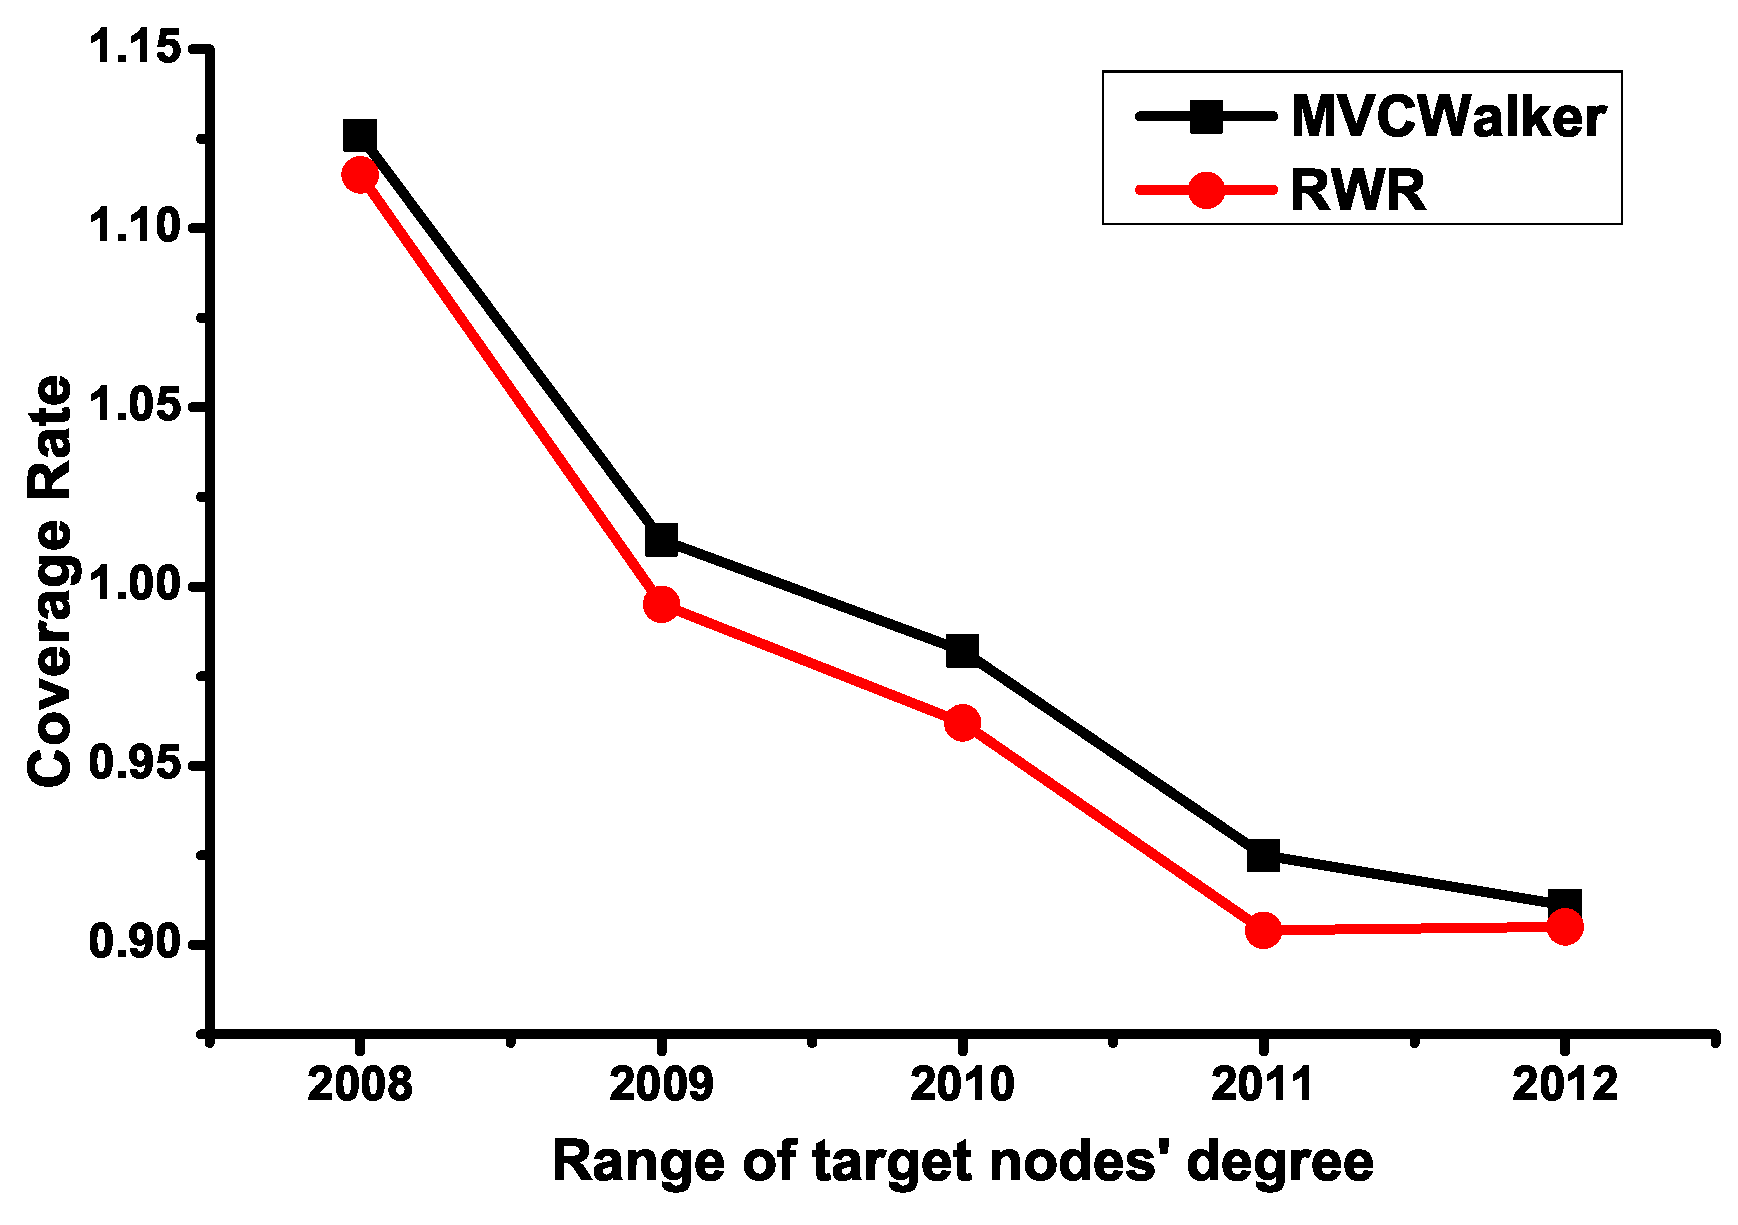
\includegraphics[width=0.31\textwidth]{Fig5-c.eps}}
\caption{Performance of MVCWalker and Basic RWR over Dataset Partitioning Time Point}
\label{fig:5}       % Give a unique label
\end{figure*}
%the social network of DBLP datasets was divided in two parts: 90\% of the data as validation set, and the remaining 10\% for testing. The first part (the large percentage of the data) was explored to create the social network and to calculate the link importance . The small part is the testing one, which means that it contains the expected results a recommender system should provide. Both parts also follow the time interval distribution, where the first part considers publications prior to the second part. In other words, the second part represents the "future" of the first one, It allows us to see what recommendations would be more accurate based on the data of the first part

The DBLP data set contains the information ranging from 1970 to 2013. In the experiments, the data set was divided into two subsets (Training Set and Test Set) by the year of publication, based on the concept of split \cite{Baeza-Yates:modern}. In this paper, we call the year as the partitioning time point. For example, the value of 2010 on X-axis in Fig. 5. means that the data before 2010 constitutes the training set while the data after 2010 make up the test set.

The effect that partitioning time point has on the performance of MVCWalker and RWR is depicted in Fig. 5. From the figures, we can see that MVCWalker performs better than RWR.

The results in Fig. 5(a) and 5(b) illustrate that both lines of precision and recall rate are similar to parabolas. In the case of MVCWalker, it recommends with higher precision and recall rate than RWR when partitioning time point ranges from 2008 to 2012. But in Fig. 5(a), the peak point is 2009, which means that when the partitioning time point is 2009, we can get the highest precision 22.5\%. While the recall rate in Fig. 5(b) gets the best performance with the value 12.3\% at the point of 2011. It is worth mentioning that, the trend of precisions for MVCWalker and RWR are similar. But for recall rate, the gap between MVCWalker and RWR is larger for the last three partitioning time points than before. In terms of coverage rate, it drops when the partitioning time point is increasing as shown in Fig. 5(c). The explanation for this is that the academic social network extracted from the data set enlarges in scale and tightens its topology, making it faster to find a collaborator when the partitioning time point increases. Fig. 5(c) validates our thought that there is a trade off between precision and coverage.

\subsubsection{Iteration Times}

\begin{figure*}
\centering
\subfigure[Precision]{
\label{fig:6-a}
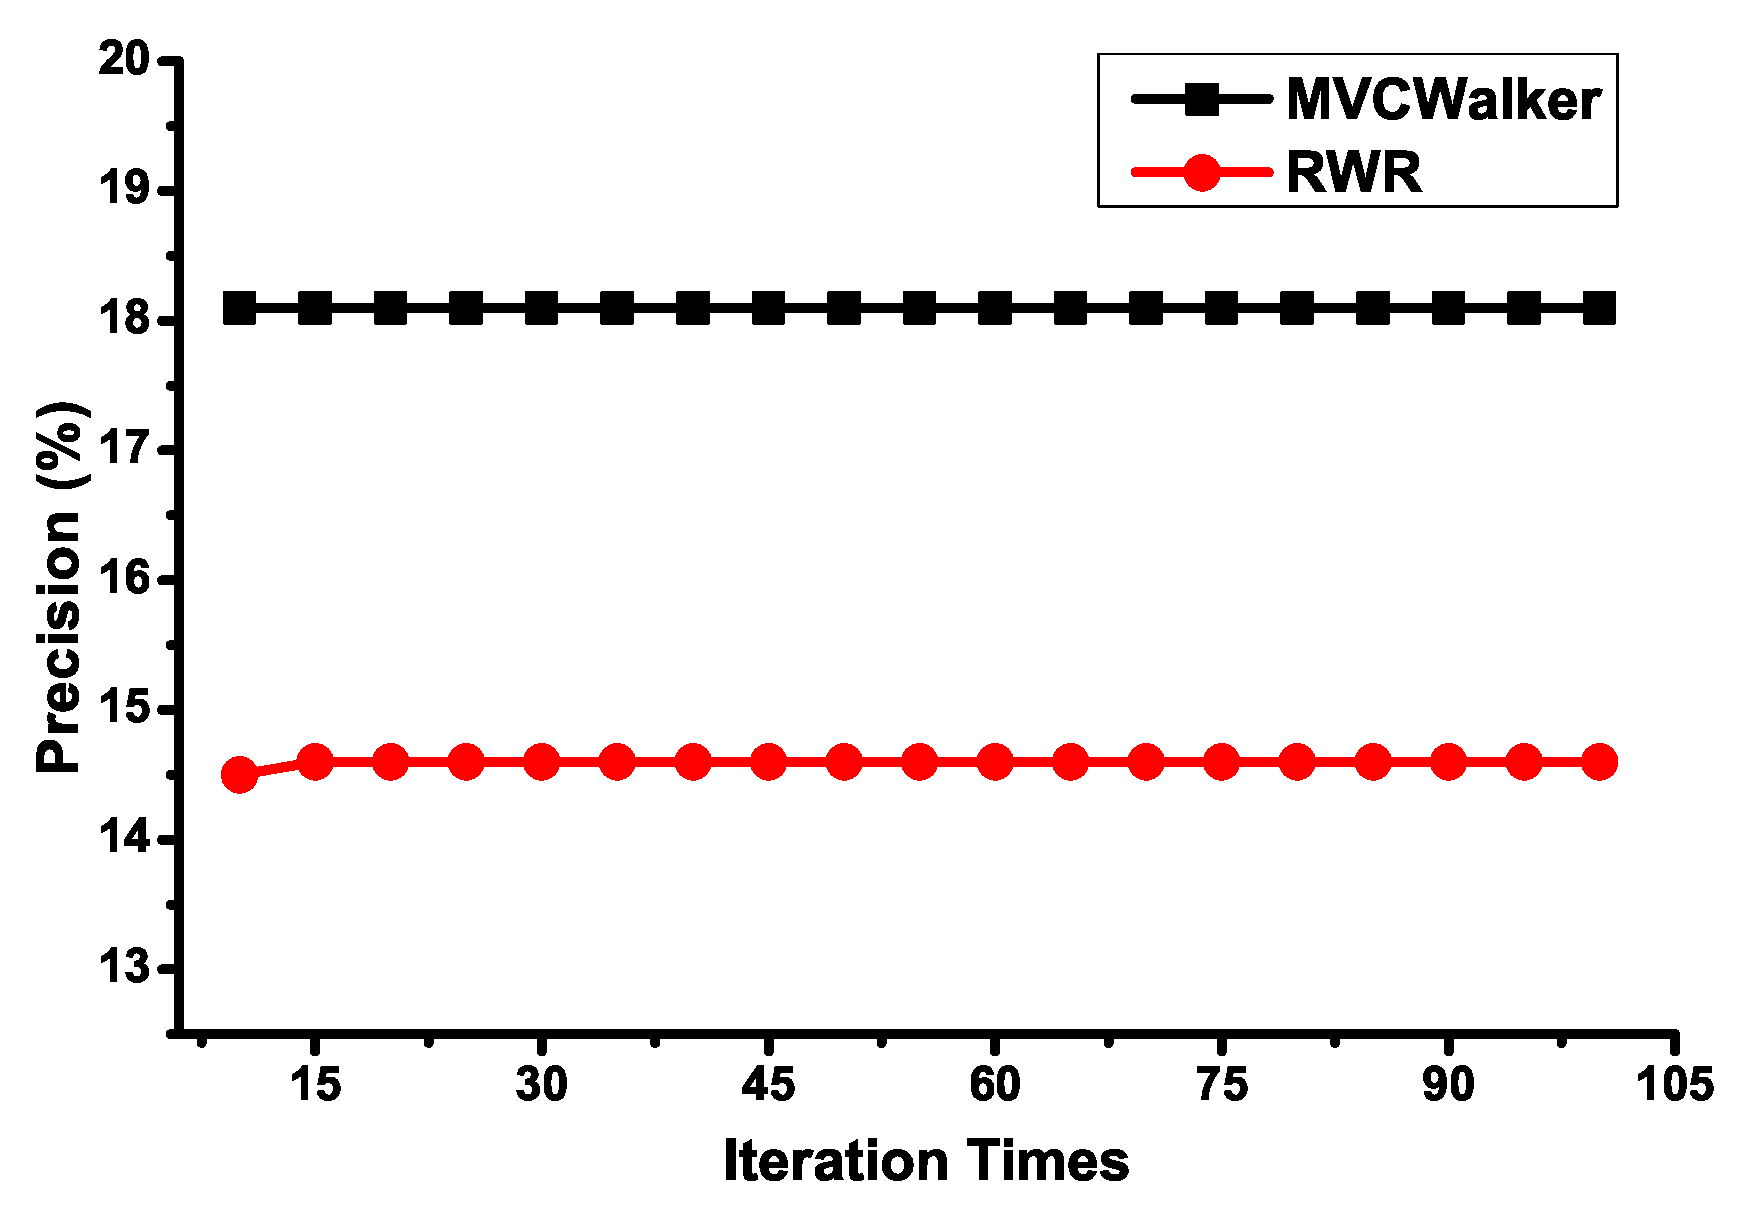
\includegraphics[width=0.31\textwidth]{Fig6-a.eps}}
\subfigure[Recall Rate]{
\label{fig:6-b}
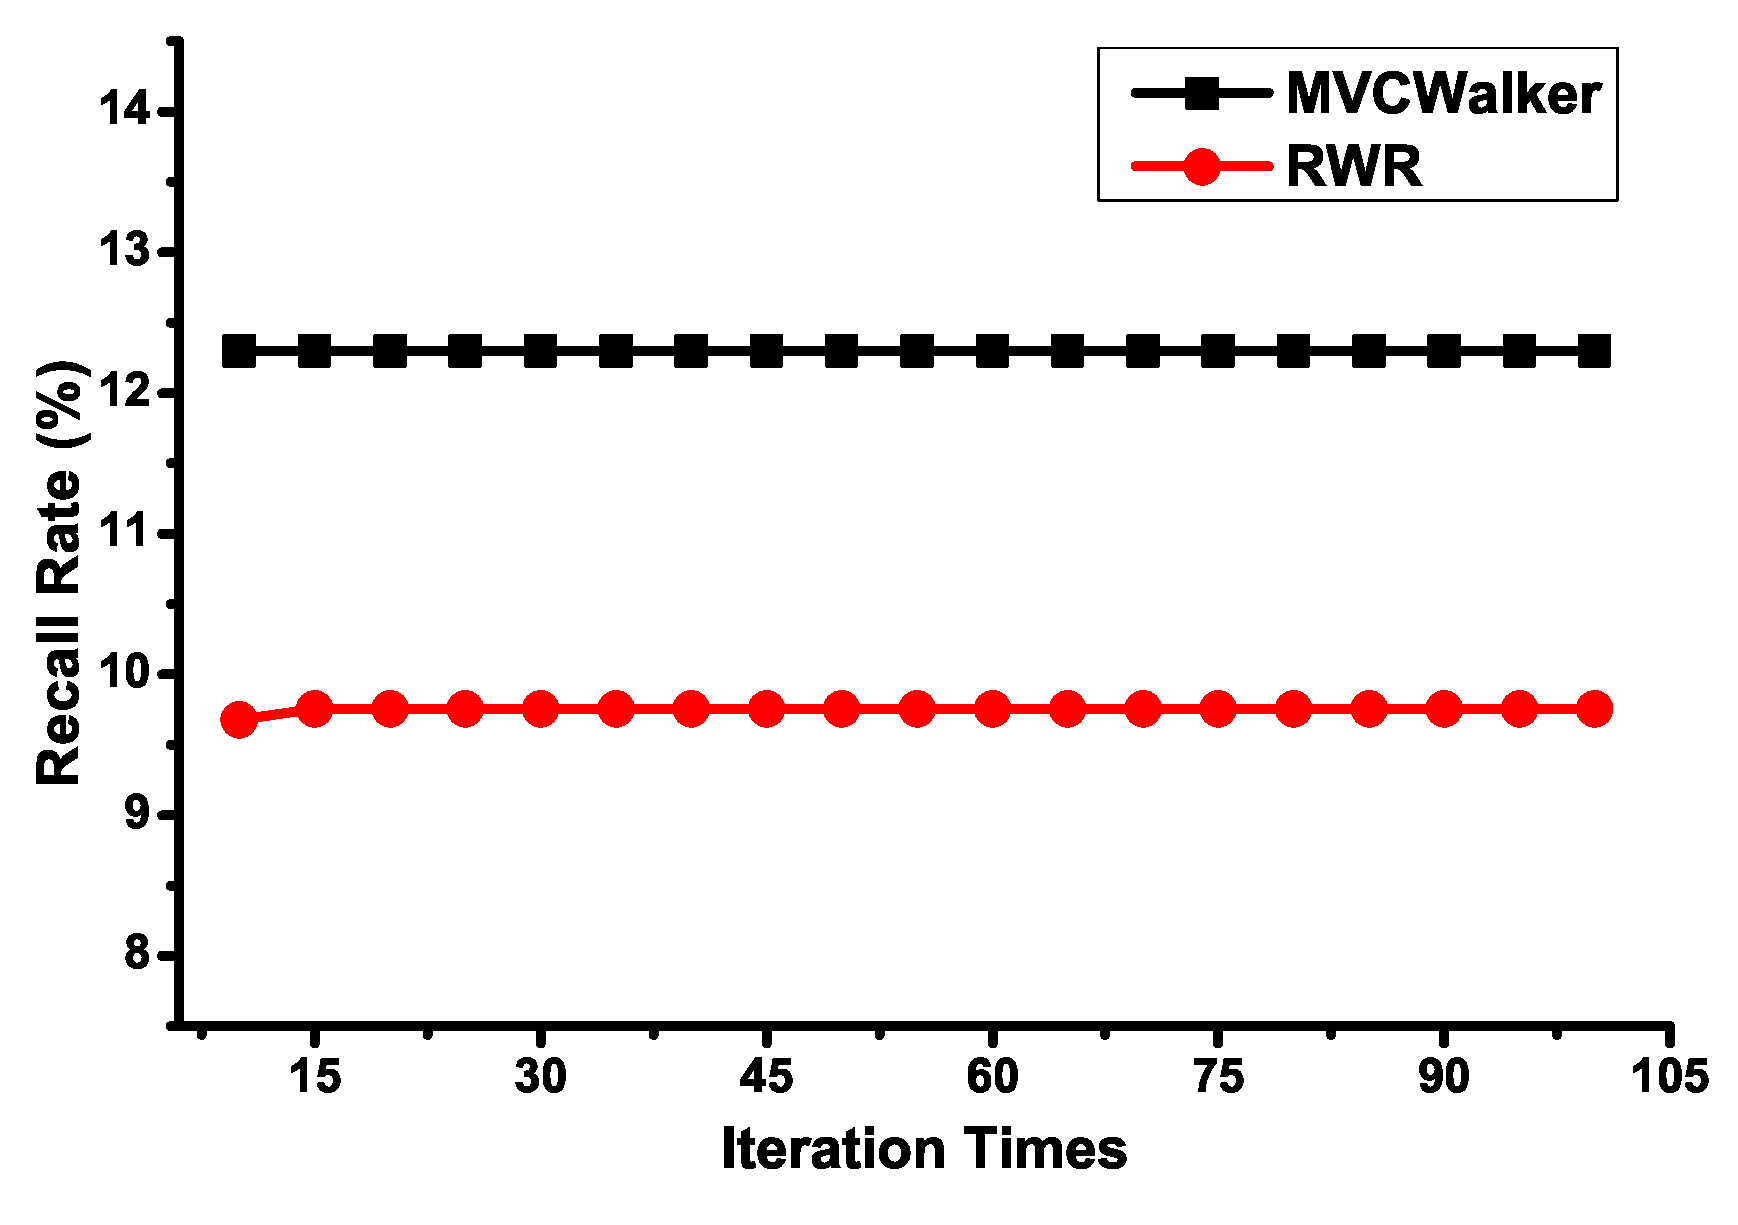
\includegraphics[width=0.31\textwidth]{Fig6-b.eps}}
\subfigure[Coverage Rate]{
\label{fig:6-c}
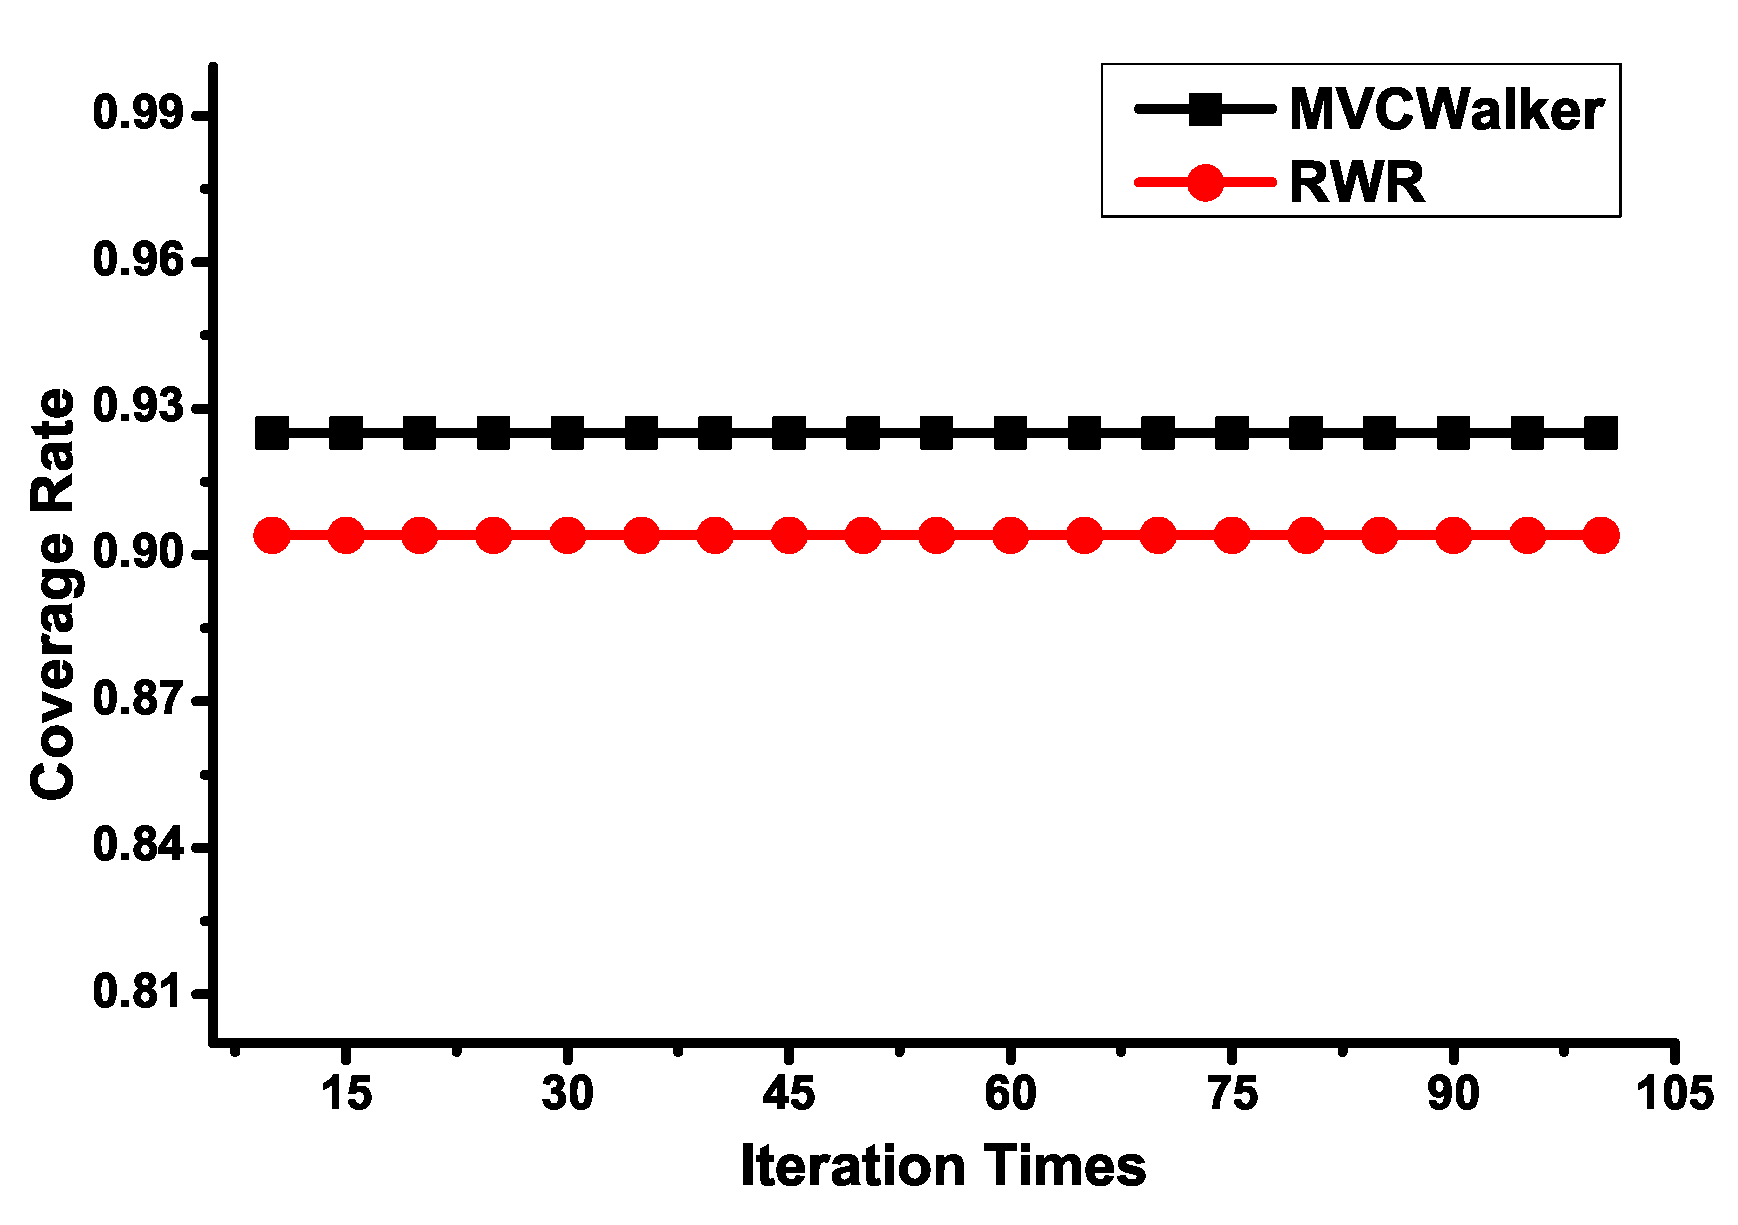
\includegraphics[width=0.31\textwidth]{Fig6-c.eps}}
\caption{Performance of MVCWalker and Basic RWR over Iteration Times}
\label{fig:6}       % Give a unique label
\end{figure*}

Fig. 6 describes the performance of recommendation under different iteration times, which represent the number of matrix multiplication operations in the relevant equation. A higher number of iterations means that the random walk will conduct more matrix multiplication operations before getting the recommended list.

The three sub-figures share one feature in common. The three metrics show no significant changes when the iteration times get bigger. But after having a close-up view of the results, we can come up with some details. In the case of RWR, according to Fig. 6(a) and Fig. 6(b), both precision and recall rate are lower than common values until 15 iteration times, then the lines become horizontal. The common values of precision and recall rate are respectively 14.6 \% and 9.76\%, which means that after the random walker conducts 15 times matrix multiplication operations, the MR will become convergent. So we don't need to execute too many iterations. Since several nodes are not able to converge in fewer iterations, we set the iteration times to 25.

\subsubsection{Damping Coefficient}

\begin{figure*}
\centering
\subfigure[Precision]{
\label{fig:7-a}
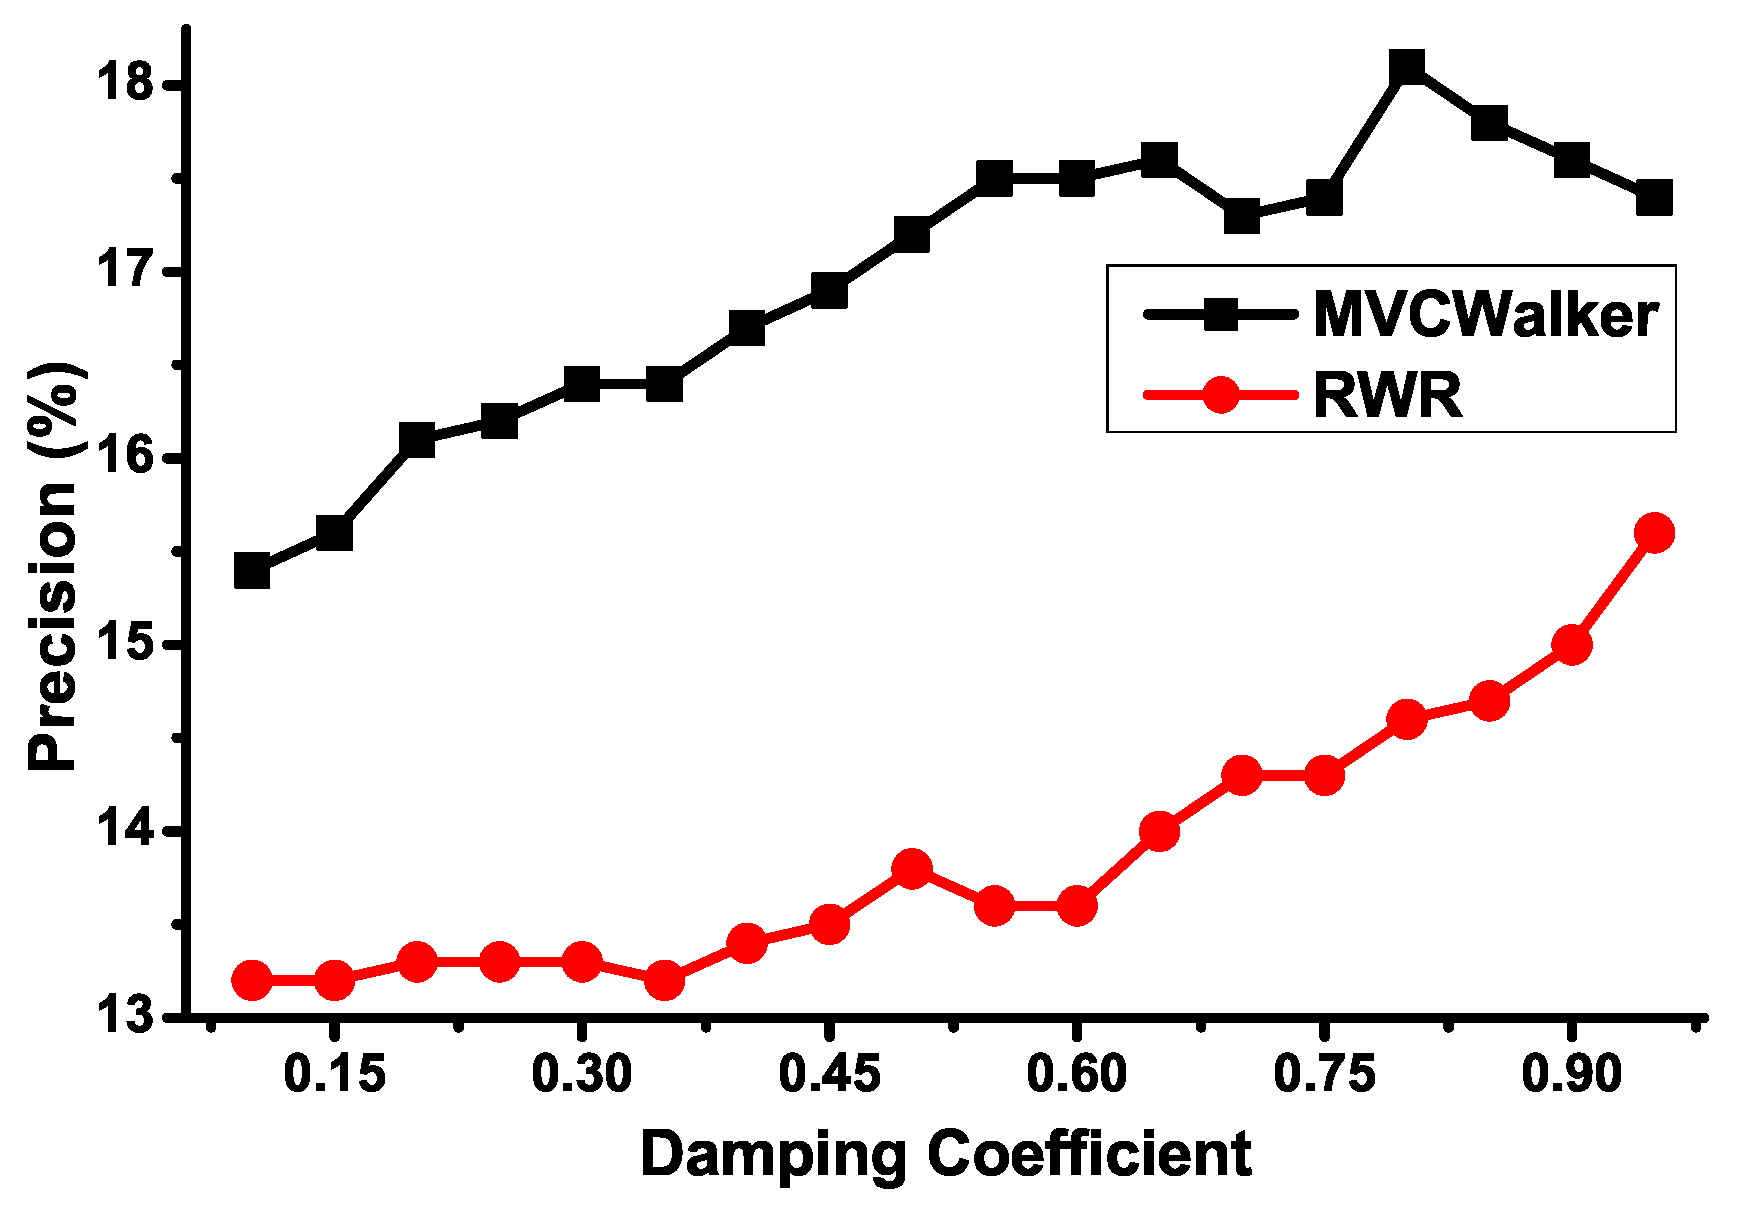
\includegraphics[width=0.31\textwidth]{Fig7-a.eps}}
\subfigure[Recall Rate]{
\label{fig:7-b}
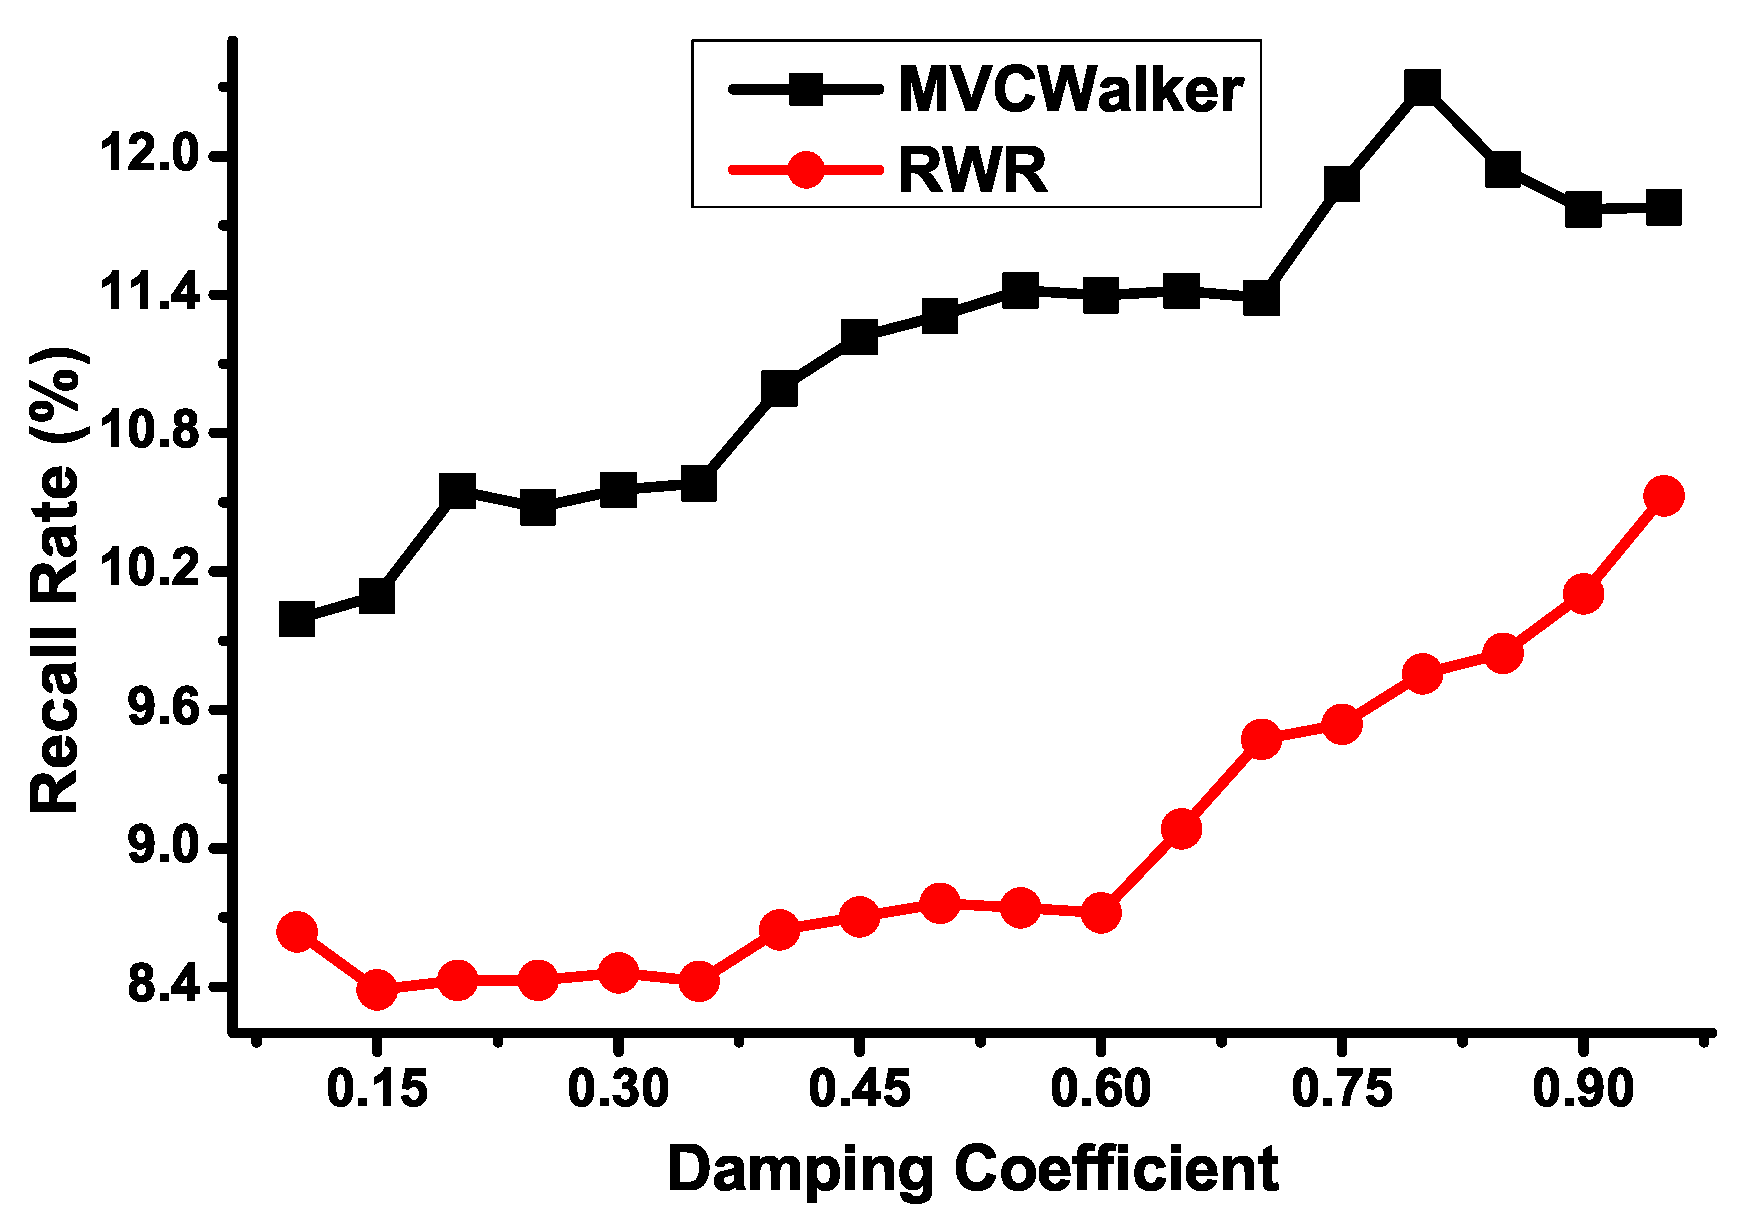
\includegraphics[width=0.31\textwidth]{Fig7-b.eps}}
\subfigure[Coverage Rate]{
\label{fig:7-c}
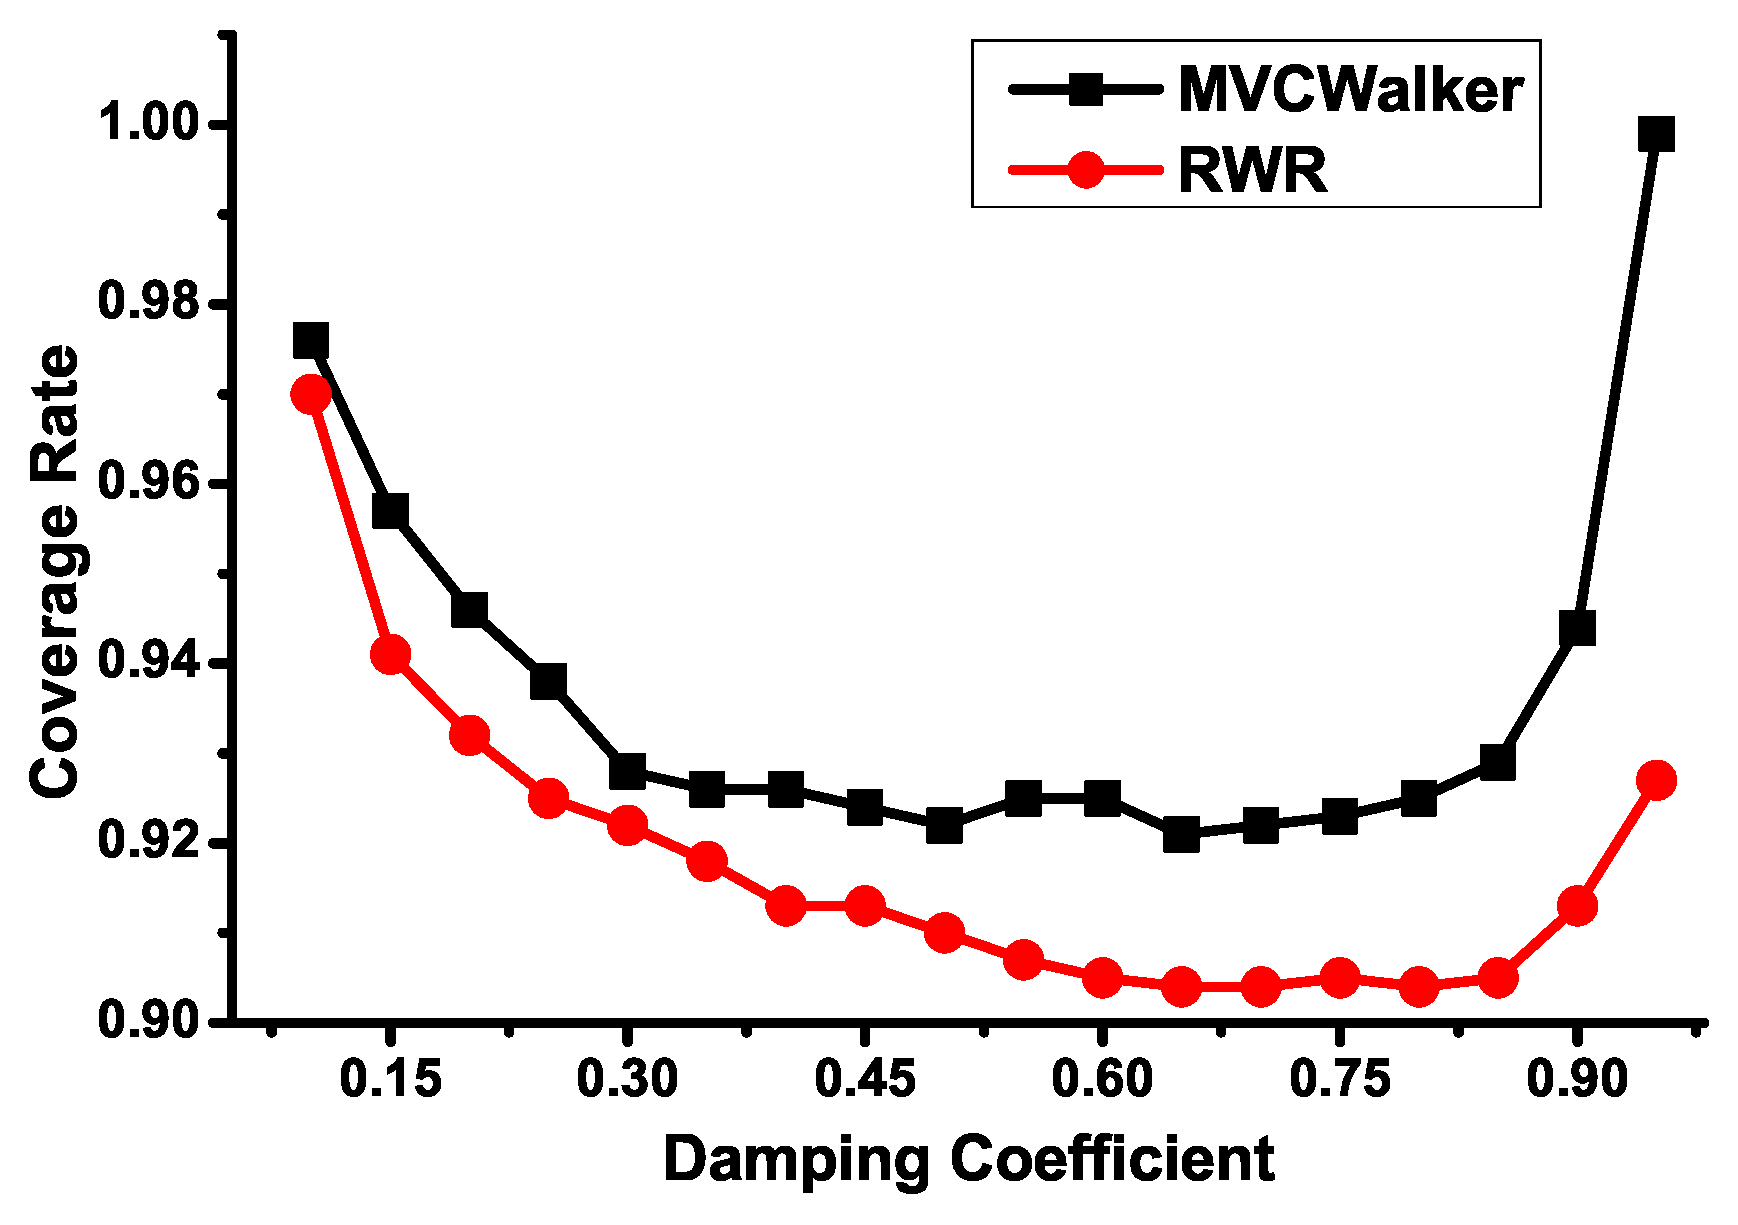
\includegraphics[width=0.31\textwidth]{Fig7-c.eps}}
\caption{Performance of MVCWalker and Basic RWR over Damping Coefficient}
\label{fig:7}       % Give a unique label
\end{figure*}

\begin{figure*}
\centering
\subfigure[Precision]{
\label{fig:8-a}
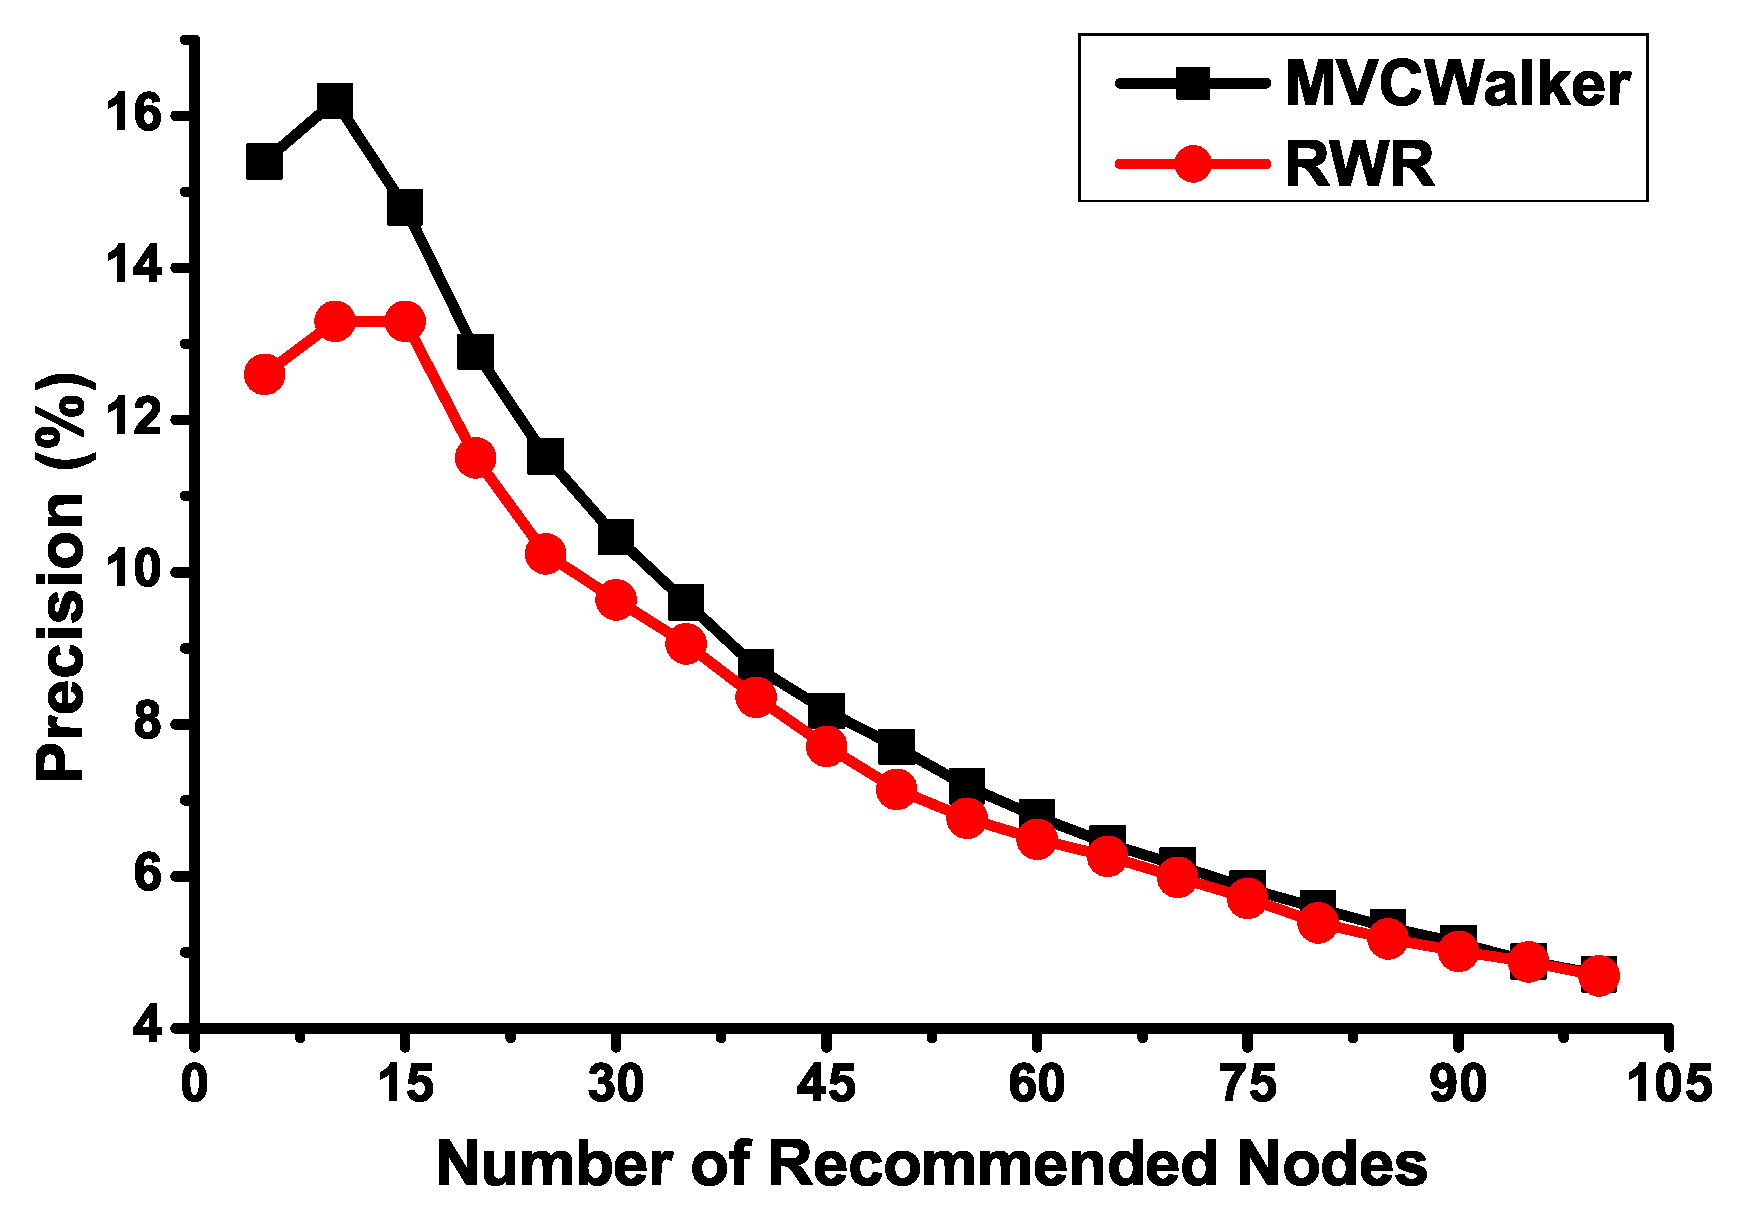
\includegraphics[width=0.31\textwidth]{Fig8-a.eps}}
\subfigure[Recall Rate]{
\label{fig:8-b}
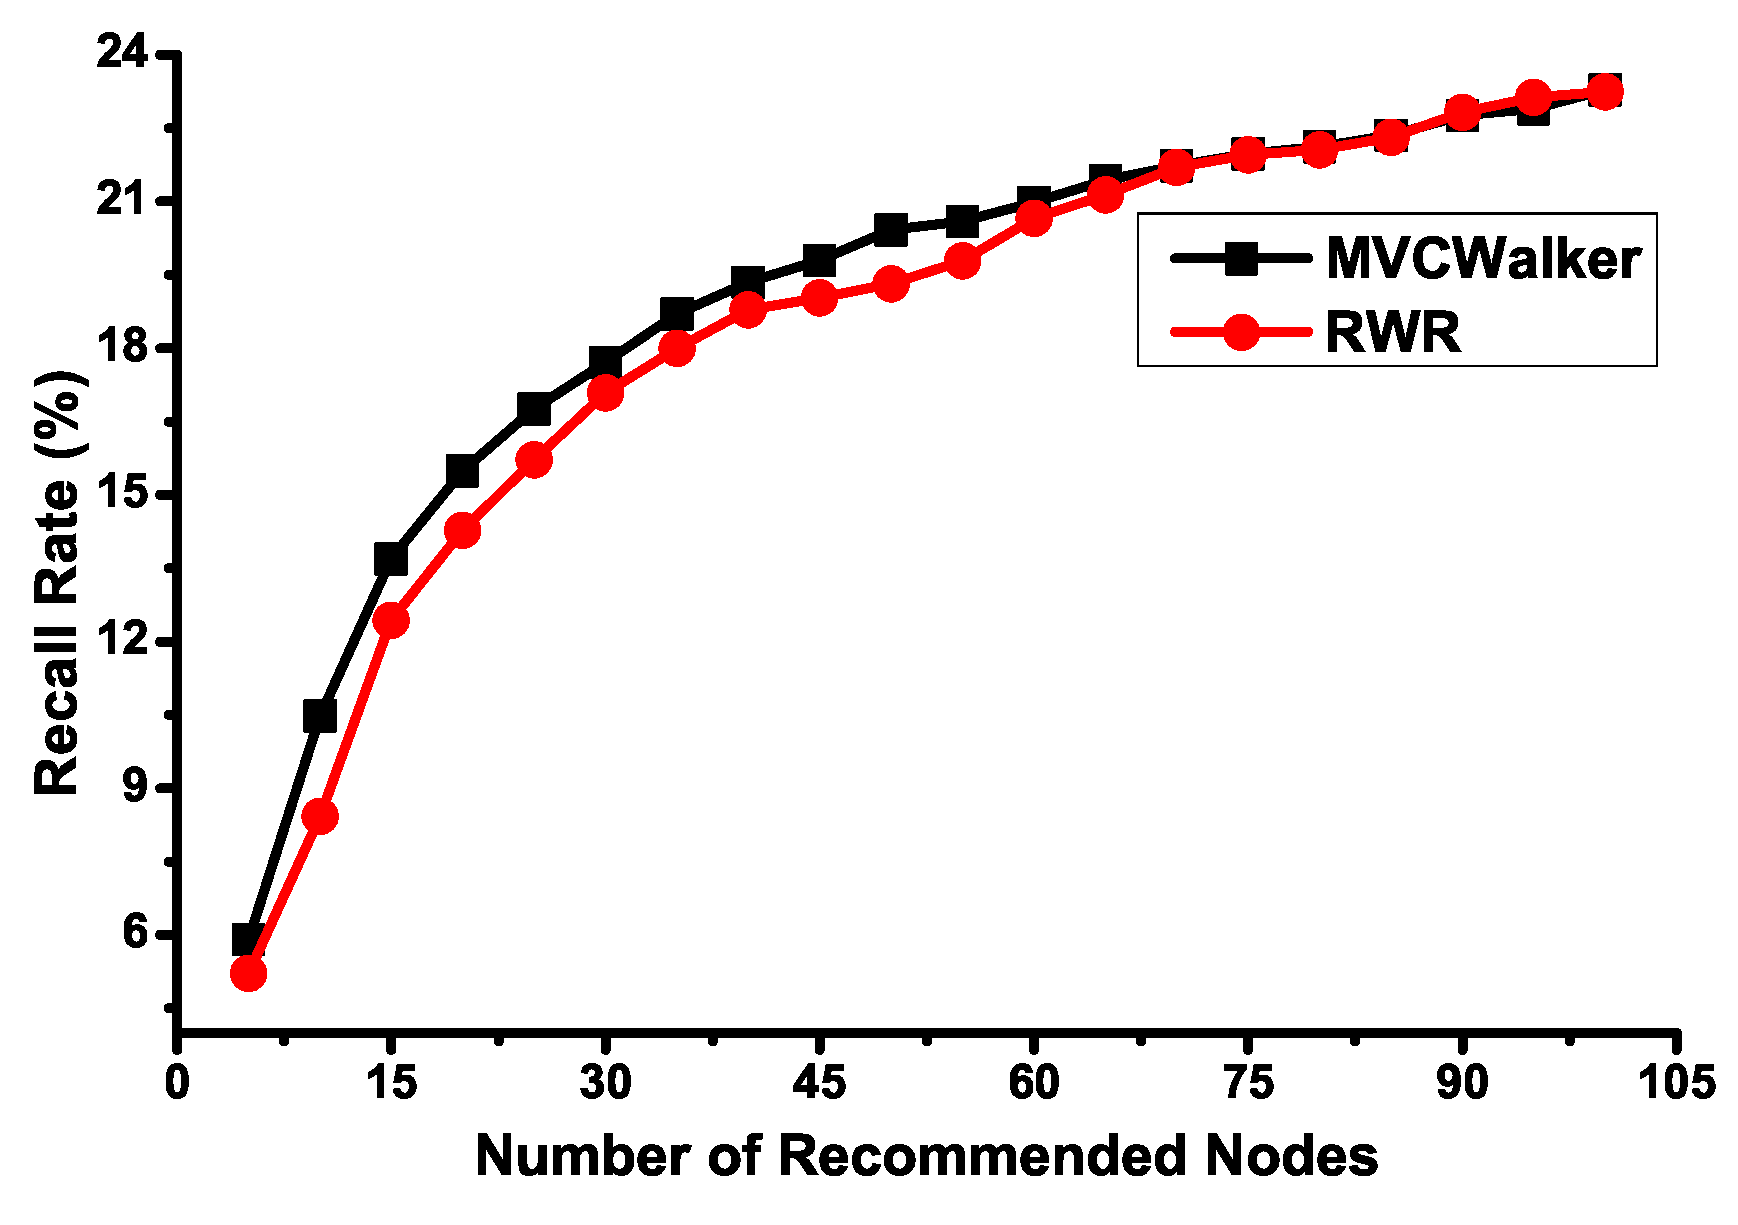
\includegraphics[width=0.31\textwidth]{Fig8-b.eps}}
\subfigure[Coverage Rate]{
\label{fig:8-c}
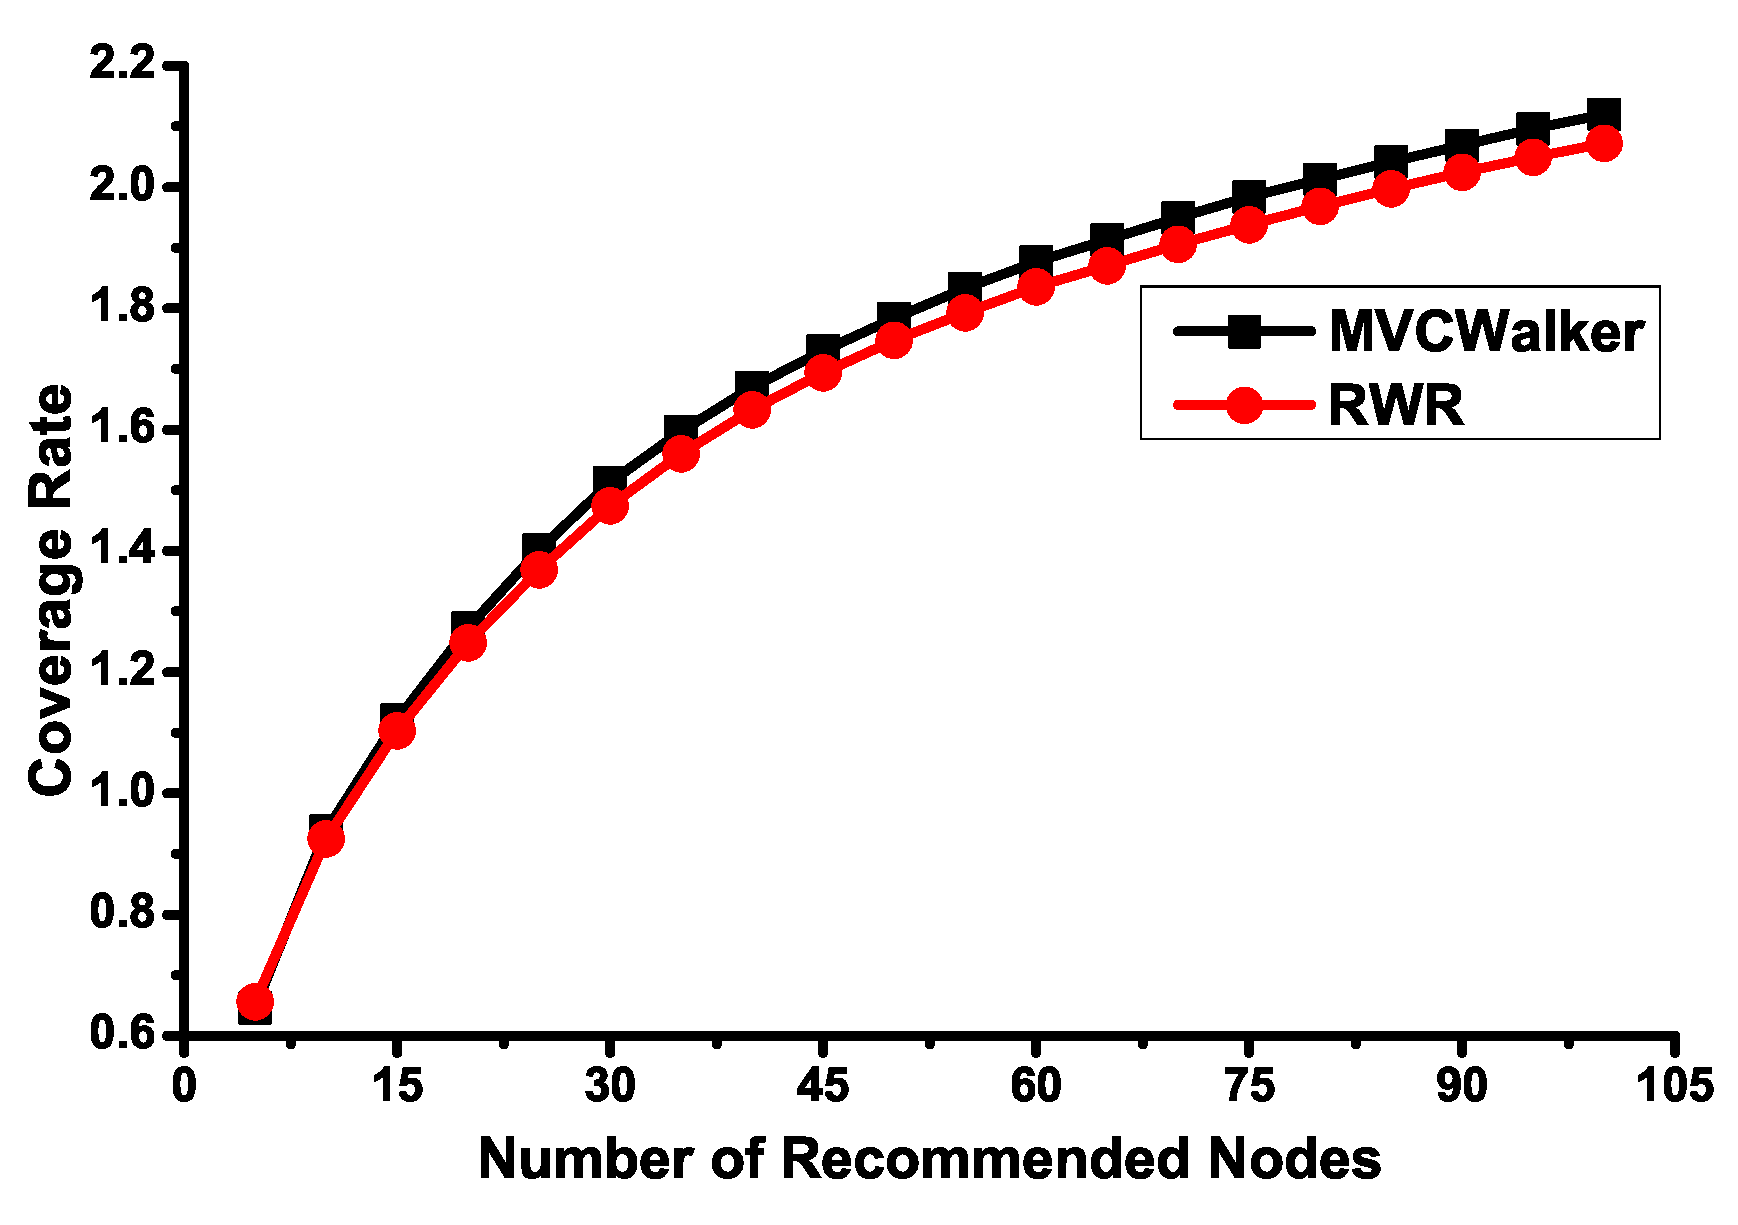
\includegraphics[width=0.31\textwidth]{Fig8-c.eps}}
\caption{Performance of MVCWalker and Basic RWR over Number of Recommended Nodes}
\label{fig:8}       % Give a unique label
\end{figure*}
In Random Walk model, there is a damping coefficient, which is usually set to 0.85, e.g. in PageRank. According to Equation (3), the value of damping coefficient determines the probability of the walker continuing walking to the next neighbor. This parameter has a realistic significance as it controls how far the MR value will be dispersed. In this section, we analyze how the damping coefficient influences the performance of the two algorithms in terms of the three metrics.

Generally, as depicted in Fig. 7, MVCWalker and RWR almost share the same trend for the majority of tested data, while MVCWalker keeps recommending with higher precision, recall rate and coverage rate, as compared against the RWR approach. Thus we prefer to focus on describing the features of MVCWalker, instead of both of them.

Fig. 7(a) shows that the influence of damping coefficient on precision is significant. We can see that, the precisions are generally increasing with the growth of damping coefficient. In the case of MVCWalker, it can be as high as 18.1\%, corresponding to the damping coefficient of 0.8. In the case of RWR, we can find that the precision is also high at this point. According to Fig. 7(b), the recall rate reaches the highest value of 12.3\% when the damping coefficient is 0.8. From Fig. 7(a) and Fig. 7(b) we can see that both precision and recall rate decrease when damping coefficient becomes larger than 0.8 for MVCWalker. Moreover, from Fig. 7(c), we can see that the coverage rate generally decreases until the damping coefficient is over 0.8, and then increases rapidly. Since the point 0.8 is exactly the peak of precision and recall rate for MVCWalker, it can be verified again that there is a trade-off between recommendation precision, recall rate and coverage. Considering the importance of precision and recall rate, we regard 0.8 as a better damping coefficient for MVCWalker.

\subsubsection{Number of Recommended Nodes}

Fig. 8 illustrates how the number of recommended nodes influences the performance of MVCWalker and RWR with respect to precision, recall rate and coverage rate.

Fig. 8(a) shows the trend of precision. We can easily find that the precision decreases dramatically with the number of recommended nodes increasing. The highest precision of MVCWalker is 16.2\% when we recommend 10 nodes to a target node while the highest precision of RWR is 13.3\% when we return a 10-node recommendation list. The reason behind this is that according to Equation (7), if we recommend more nodes, both the values of $A$ and $C$ rise, but $C$ grows faster than $A$, resulting in the precision becomes smaller.

In terms of the performance of recall rate, Fig. 8(b) shows that the recall rate increases gradually. The result is opposite to that of precision. According to Equation (8), the increase of the number of recommended nodes makes $A$ grow while $(A+B)$ remains the same. Consequently, the recall rate increases.

Fig. 8(c) also depicts clearly that precision is almost inverse to coverage. Additionally, it is shown by the figure that MVCWalker performs slightly better than RWR.

\subsection{Comparison with Other Methods}

\begin{figure}
%\centering
\subfigure[Precision]{
\label{fig:9-a}
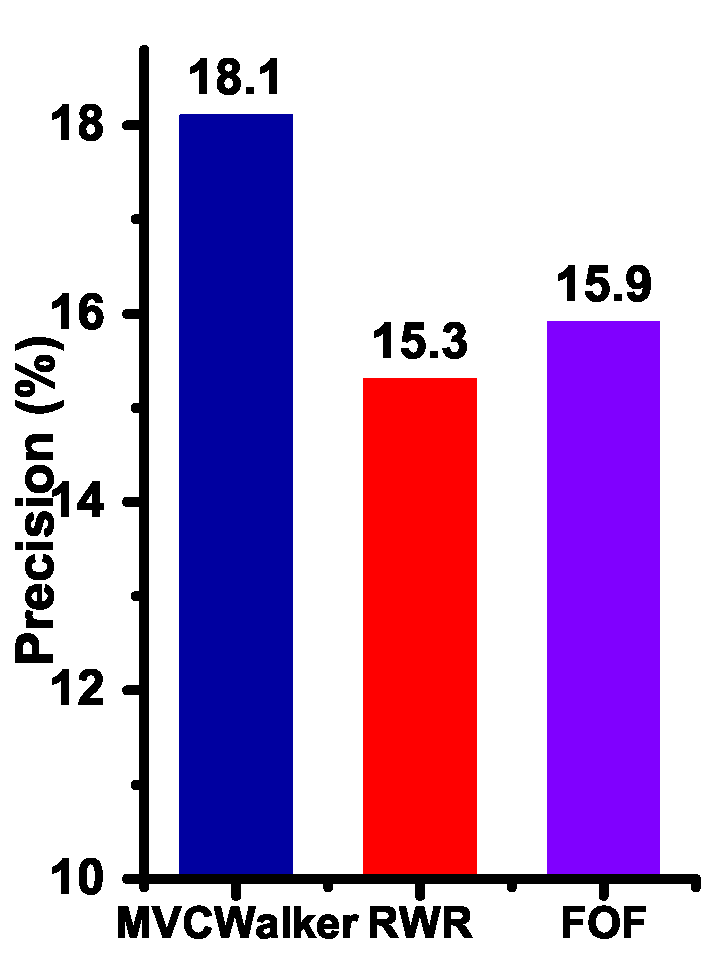
\includegraphics[width=0.14\textwidth]{Fig9-a.eps}}
\subfigure[Recall Rate]{
\label{fig:9-b}
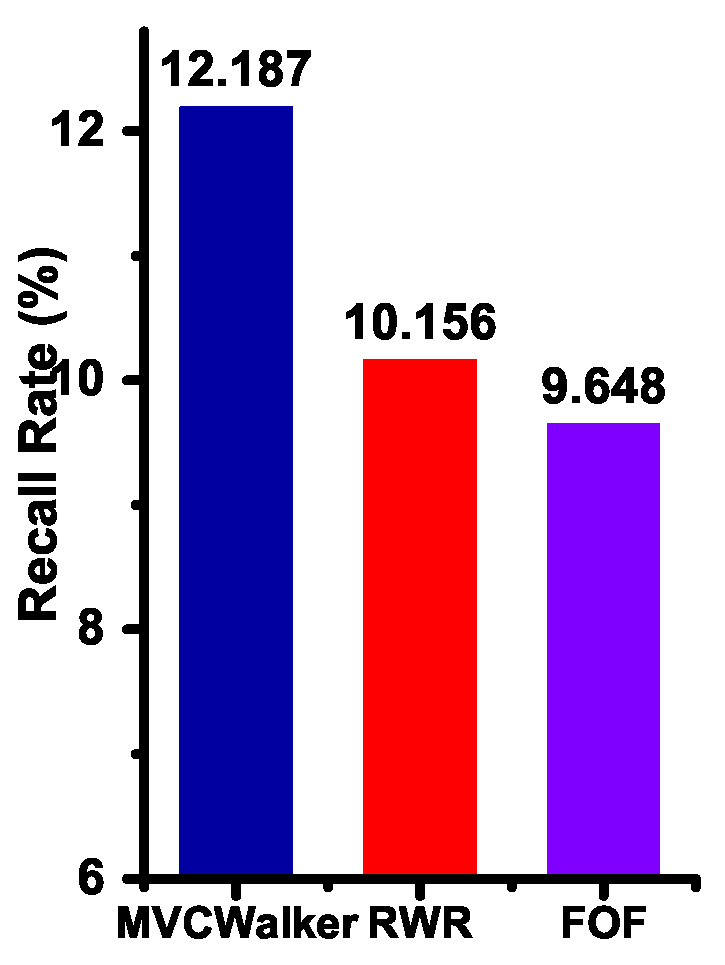
\includegraphics[width=0.14\textwidth]{Fig9-b.eps}}
\subfigure[Coverage Rate]{
\label{fig:9-c}
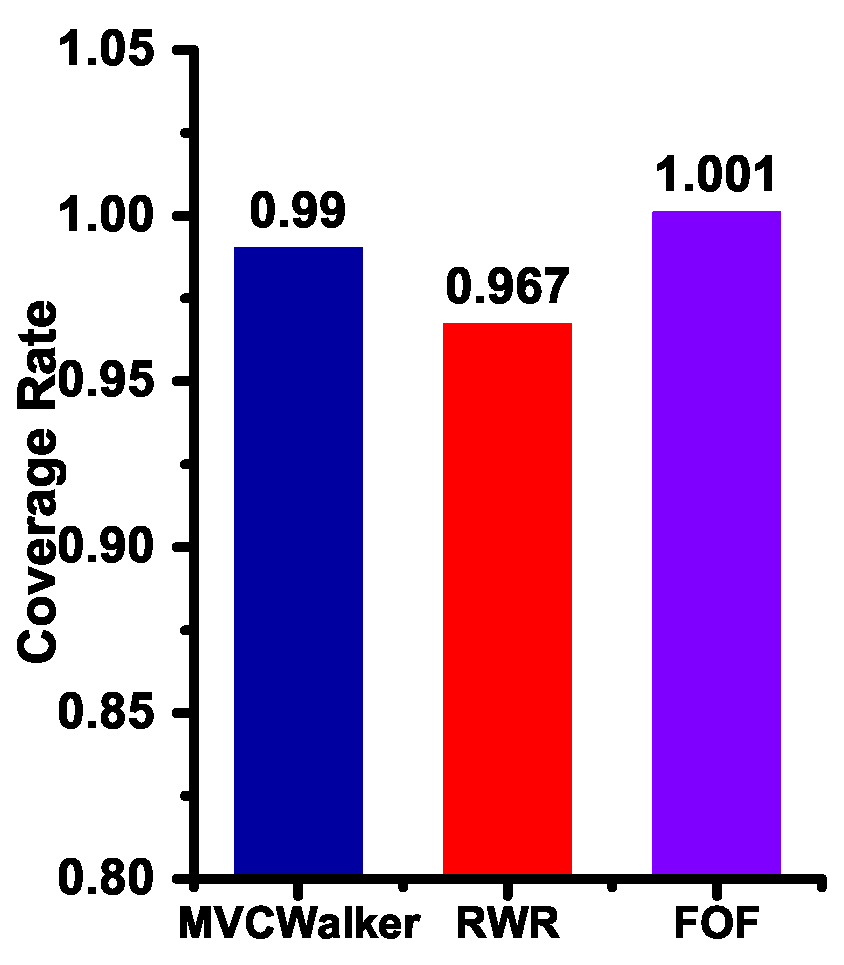
\includegraphics[width=0.155\textwidth]{Fig9-c.eps}}
\caption{Comparison of MVCWalker, RWR and FOF}
\label{fig:9}       % Give a unique label
\end{figure}

As can be seen from the experiments above, the consideration of academic social factors (i.e. coauthor order, latest collaboration time point and collaboration times) helps MVCWalker recommend more precisely with higher recall rate, in a wider scope in a coauthor network, and it performs better than the benchmark model RWR. Besides, the parameters we take into account affect the performance in diverse manners and we have found their best values for MVCWalker.

We carry out experiments to compare the performance of MVCWalker, RWR and FOF. We run 100 times for each model, and keep the 100 target nodes same for each model. The MVCWalker and RWR are conducted over the five optimized parameters in previous experiments, i.e. target node's degree: $>30$; partitioning time point: 2011; iteration times: 25; damping coefficient: 0.8; and number of recommended nodes: 10.

The results are shown in Fig. 9. The precision of MVCWalker is $18.1\%$, in comparison to $15.3\%$ of RWR and $15.9\%$ of FOF. In the case of recall rate, MVCWalker has the best value, $12.187\%$, which is higher than the recall rate of RWR and FOF, i.e. $10.156\%$ and $9.648\%$ respectively. It is clear that both precision and recall rate of MVCWalker are higher than those of RWR and FOF. Moreover the precision of FOF is a little higher than that of RWR, but its recall rate is a little lower than RWR. The coverage rate of MVCWalker is not so good as the first two indicators, better than that of RWR for our optimizing and lower than that of FOF. However, as can be seen in Fig. 9. the differences between their coverage rates are very small.

One more thing worth noting is the time complexity. We run 100 times for each model, and record the average running time. In FOF, making recommendation one time spend 1.2 seconds on average, in comparison to 3 seconds in both MVCWalker and RWR. According to Section 3.3, to acquire the value of LIM, MVCWalker does more extra computation than RWR, but why is the recommendation efficiency similar? This is because the guidance work in MVCWalker can enable the walker to encounter the most valuable node quicker and make the iteration stop at a faster rate, which we can identify in Fig. 6, the lines for MVCWalker become smooth earlier. In terms of time complexity, MVCWalker are not dominant as compared to FOF. But for most recommendation system, this disadvantage in time complexity is acceptable and does not much affect the recommendation effectiveness.

In summary, we can still claim that the three factors we explore perform quite well, and MVCWalker is more effective than RWR and FOF in terms of its precision and recall rate.

%\begin{figure}
%\centering
%\subfigure[Precision]{
%\label{fig:9-a}
%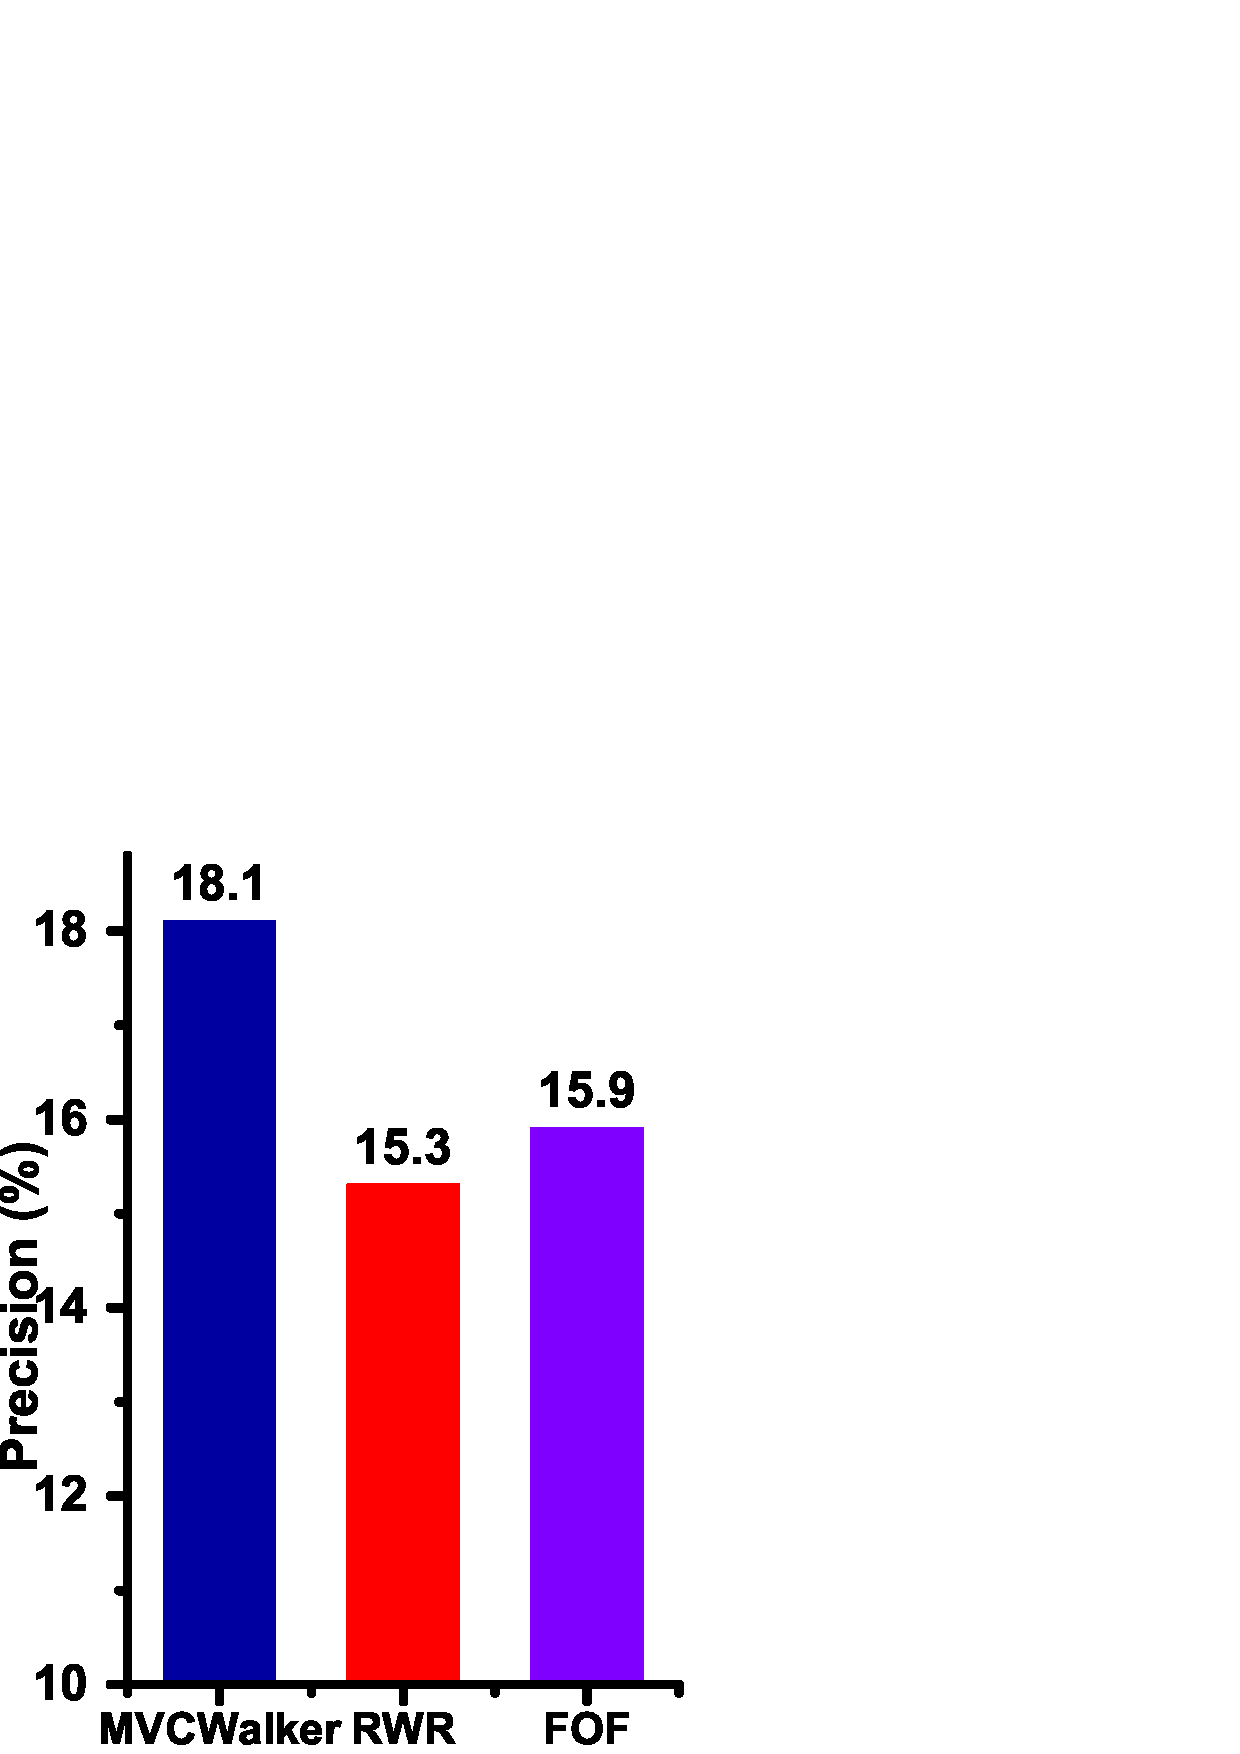
\includegraphics[width=3in]{Fig9-a.jpg}}
%\subfigure[Recall Rate]{
%\label{fig:9-b}
%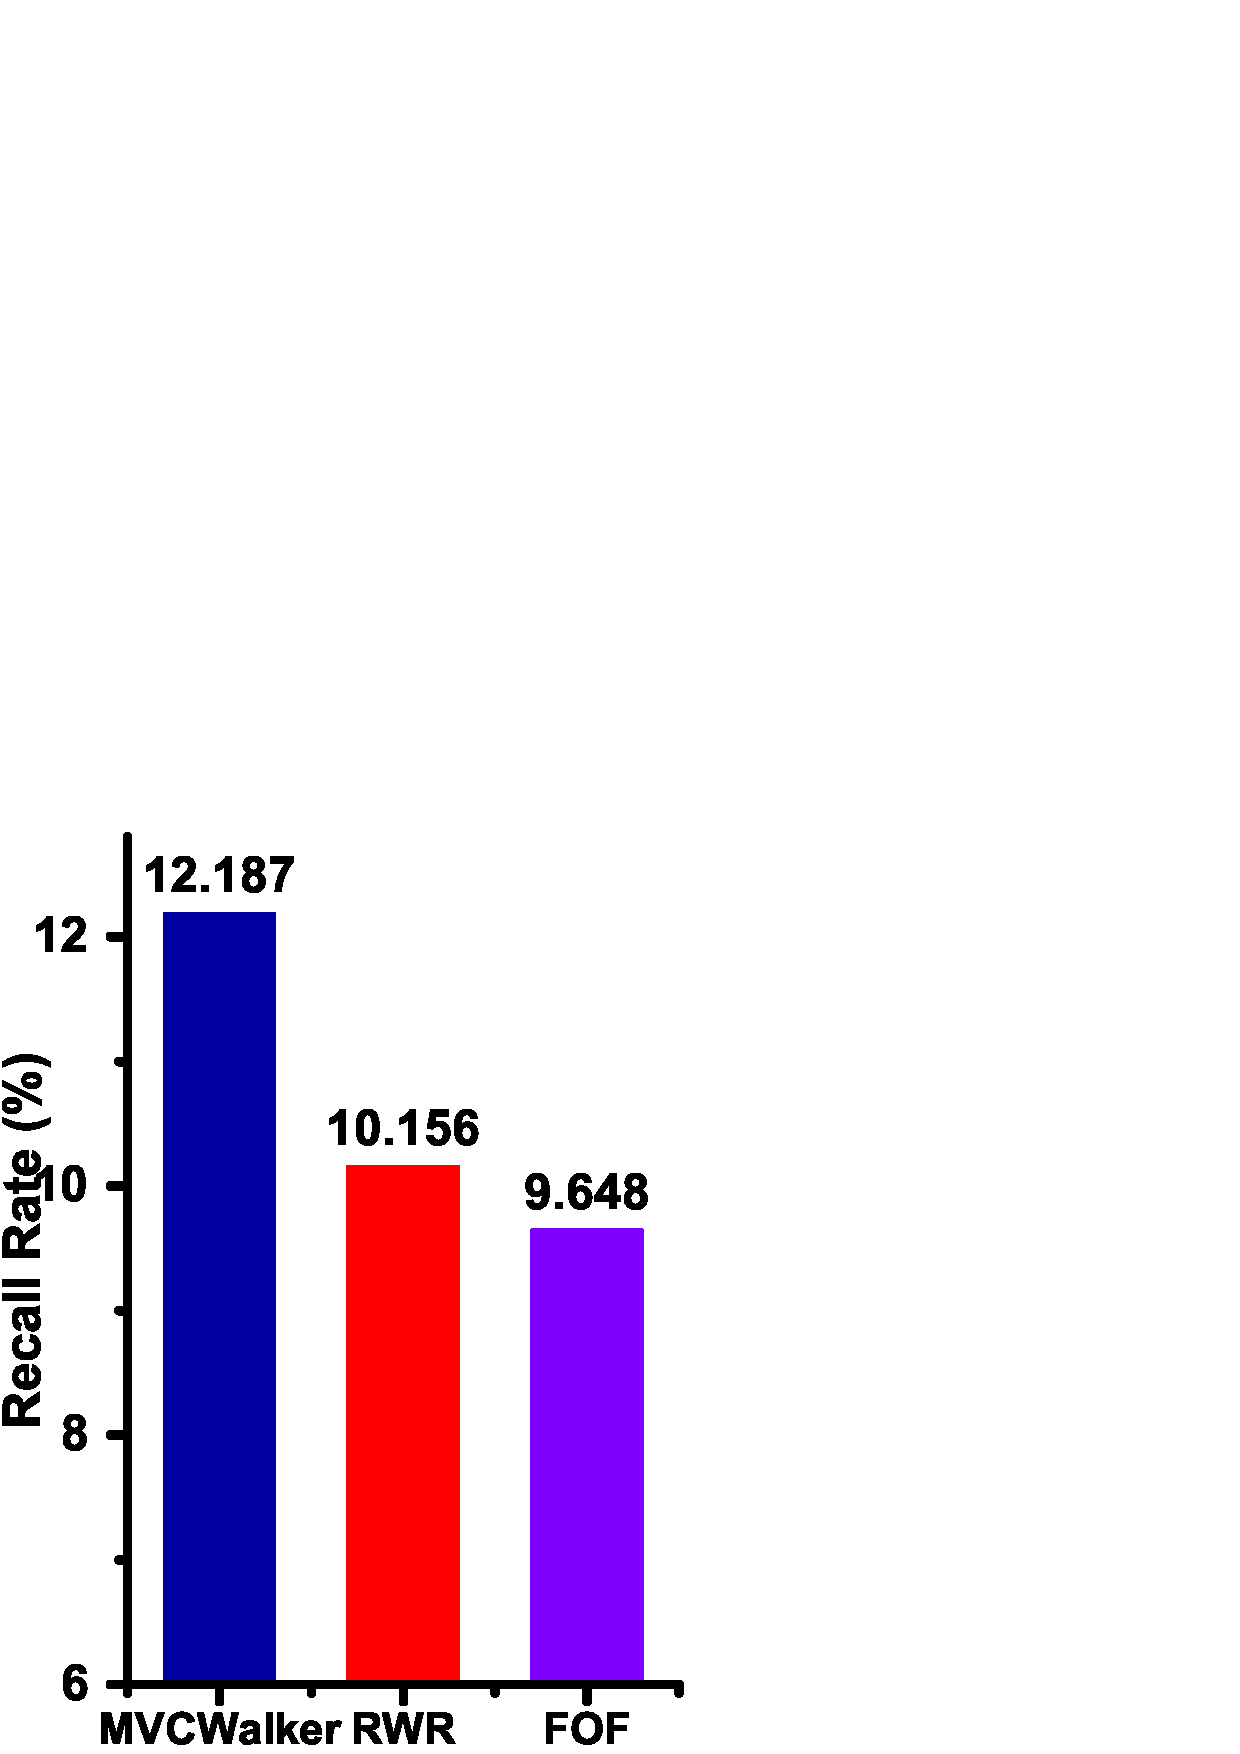
\includegraphics[width=3in]{Fig9-b.jpg}}
%\caption{Performance of MVCWalker and Basic RWR Tested on the Entire DBLP Data Set. The red line or dots in each sub-figure refers to data about MVCWalker, and the blue ones %correspond to RWR. }
%\label{fig:12}       % Give a unique label
%\end{figure}


\section{Conclusion}
In this paper, we focused on how to find scholars' MVCs based on coauthor networks (i.e. big scholarly data) which is rarely studied in the literature. To this end, we have proposed a new model named MVCWalker, by injecting three academic factors into RWR. These factors are coauthor order, latest collaboration time point and collaboration times, constituting the weight of link importance between two authors for recommendation. We conducted extensive experiments on a subset of DBLP data set to examine the performance of MVCWalker with respect to various aspects, such as varying parameters and impact of the factors. We also conducted the RWR model and FOF model on the data set as comparisons. The experimental results show that our proposed approach performs better than RWR and FOF.

Nonetheless, there is still room for future study in this direction. We only count on three academic factors while many other features such as citation relation exist and should be explored in the direction of MVCWalker. Besides, there are more reasons for two scholars with no collaboration before to cooperate. For example, they might attend the same meeting and get acquainted to each other by chance, or they are from the same institution. The relationship among co-authors of a paper is far more complicated than what we have imagined. As a future work, more experiments on the entire DBLP data set could be conducted.

%\section*{Acknowledgments}
%
%The authors would like to thank...


% Can use something like this to put references on a page
% by themselves when using endfloat and the captionsoff option.
\ifCLASSOPTIONcaptionsoff
  \newpage
\fi

\bibliographystyle{IEEEtr}
\bibliography{mvcwalker}
% biography section
%
% If you have an EPS/PDF photo (graphicx package needed) extra braces are
% needed around the contents of the optional argument to biography to prevent
% the LaTeX parser from getting confused when it sees the complicated
% \includegraphics command within an optional argument. (You could create
% your own custom macro containing the \includegraphics command to make things
% simpler here.)
\begin{biography}[{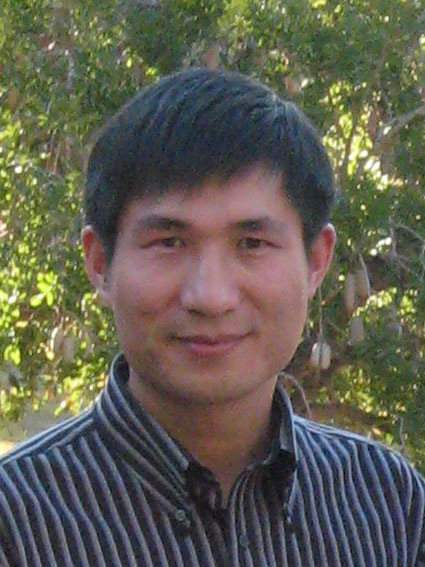
\includegraphics[width=1in,height=1.25in]{FengXia.jpg}}]{Feng Xia} (M��07-SM��12) received the BSc and Ph.D. degrees from Zhejiang University, Hangzhou, China, in 2001 and 2006, respectively. He is an Associate Professor and PhD Supervisor in School of Software, Dalian University of Technology, China. He is the (Guest) Editor of several international journals. He serves as General Chair, PC Chair, Workshop Chair, Publicity Chair, or PC Member of a number of conferences. Dr. Xia has authored/co-authored one book and over 160 scientific papers in international journals and conferences. His research interests include social computing, mobile computing, and cyber-physical systems. He is a Senior Member of IEEE and a member of ACM.
\end{biography}

\begin{biography}[{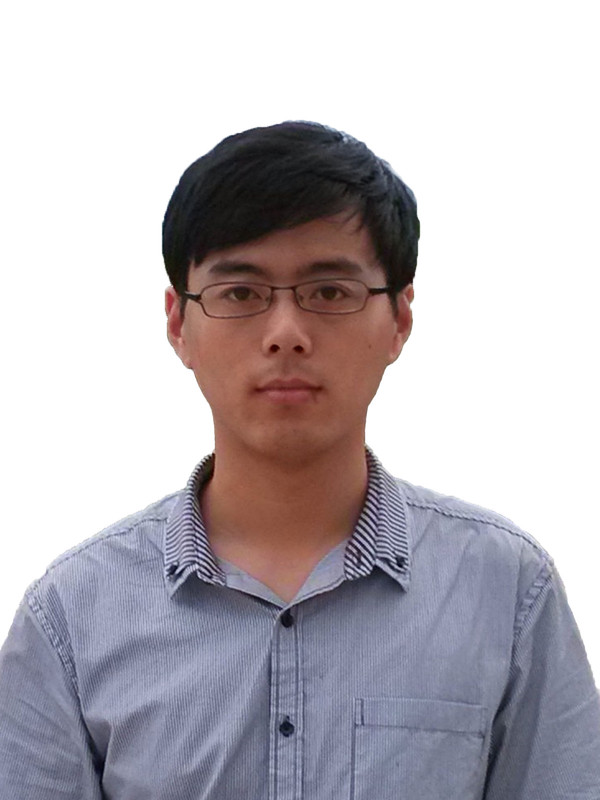
\includegraphics[width=1in,height=1.25in]{ZhenChen.jpg}}]{Zhen Chen} received his B.S. degree from Dalian University of Technology (DUT), Dalian, China, in 2013. He is currently working towards the M.S. degree in Software Engineering in DUT. His research interests include recommender systems, big scholarly data, smart computing systems.
\end{biography}

\begin{biography}[{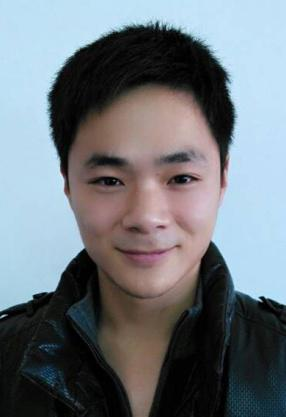
\includegraphics[width=1in,height=1.25in]{WeiWang.jpg}}]{Wei Wang} received the B.S. degree in Electronic Information Science and Technology from Shenyang University, Shenyang, China, in 2012. He is currently working towards the Ph.D. degree in Software Engineering in Dalian University of Technology (DUT), Dalian, China. His research interests include big scholarly data, social networks and computational social science.
\end{biography}

\begin{biography}[{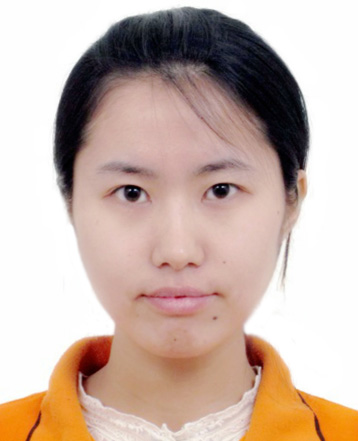
\includegraphics[width=1in,height=1.25in]{JingLi.jpg}}]{Jing Li} received B.E. degree from Dalian University of Technology, China, in 2011. Currently she is a Master student in School of Software, Dalian University of Technology. Her research interests include recommender systems, social computing, and smart meeting.
\end{biography}


\begin{biography}[{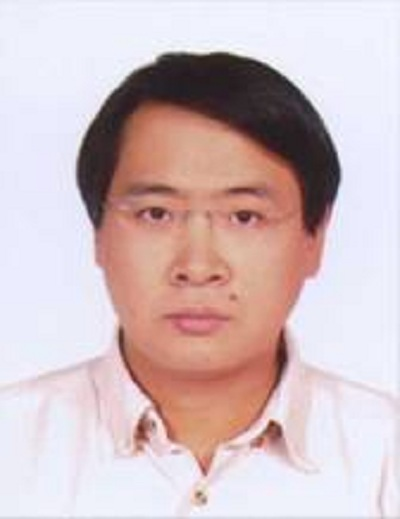
\includegraphics[width=1in,height=1.25in]{LaurenceYang.jpg}}]{Laurence T. Yang} received the BE degree in computer science and technology from Tsinghua University, China and the PhD degree in computer science from University of Victoria, Canada. He is a professor in the School of Computer Science and Technology at Huazhong University of Science and Technology, China, and in the Department of Computer Science, St. Francis Xavier University, Canada. His research interests include parallel and distributed computing, embedded and ubiquitous/pervasive computing. His research has been supported by the National Sciences and Engineering Research Council, and the Canada Foundation for Innovation.
\end{biography}


% or if you just want to reserve a space for a photo:

%\begin{IEEEbiography}{Michael Shell}
%Zhen Chen received his B.S. degree in Dalian University of Technology (DUT), Dalian, China, in 2013. He is currently working toward the M.S. degree in Software Engineering in DUT.
%His research interests include recommendation technology, big scholarly data, smart computing systems.
%\end{IEEEbiography}

%\begin{IEEEbiography}{Michael Shell}
%Wei Wang received his B.S. degree in Electronic Information Science and Technology from Shenyang University, Shenyang, China, in 2012. He is currently working toward the Ph.D. degree in Software Engineering in Dalian University of Technology (DUT), Dalian, China.
%His research interests include big scholarly data, social networks and computational social science.
%\end{IEEEbiography}

%\begin{IEEEbiography}{Michael Shell}
%Jing Li received her M.S. degree in 2014 and B.S. degree in 2011 from Dalian University of Technology (DUT), Dalian, China.
%Her research interests include recommendation technology, big scholarly data, smart computing systems.
%\end{IEEEbiography}

% You can push biographies down or up by placing
% a \vfill before or after them. The appropriate
% use of \vfill depends on what kind of text is
% on the last page and whether or not the columns
% are being equalized.

%\vfill

% Can be used to pull up biographies so that the bottom of the last one
% is flush with the other column.
%\enlargethispage{-5in}



% that's all folks

\end{document}


